 % arara: clean: { files: [thesis.aux, thesis.bbl, thesis.blg, thesis.dvi, thesis.fdb_latexmk, thesis.fls, thesis.idx, thesis.ilg, thesis.ind, thesis.lof, thesis.log, thesis.lot, thesis.nlo, thesis.nls, thesis.out, thesis.pdf, thesis.ps, thesis.toc]}
% arara: latex:  { shell: yes }
% arara: bibtex
% arara: nomencl
% arara: latex
% arara: makeindex
% arara: latex:  { shell: yes }
% arara: dvips
% arara: ps2pdf

% ******************************* PhD Thesis Template **************************
% Please have a look at the README.md file for info on how to use the template

\documentclass[a4paper,12pt,customfont,draftclassic,numbered,print,index]{PhDThesisPSnPDF}
\title{PhD Thesis}

% ******************************************************************************
% ******************************* Class Options ********************************
% *********************** See README for more details **************************
% ******************************************************************************

% `a4paper'(The University of Cambridge PhD thesis guidelines recommends a page
% size a4 - default option) or `a5paper': A5 Paper size is also allowed as per
% the Cambridge University Engineering Deparment guidelines for PhD thesis
%
% `11pt' or `12pt'(default): Font Size 10pt is NOT recommended by the University
% guidelines
%
% `oneside' or `twoside'(default): Printing double side (twoside) or single
% side.
%
% `print': Use `print' for print version with appropriate margins and page
% layout. Leaving the options field blank will activate Online version.
%
% `index': For index at the end of the thesis
%
% `draft': For draft mode without loading any images (same as draft in book)
%
% `draftmode': Special draft mode with line numbers, images, and water mark with
% timestamp and custom text. Position of the text can also be modified.
%
% `abstract': To generate only the title page and abstract page with
% dissertation title and name, to submit to the Student Registry
%
% `chapter`: This option enables only the specified chapter and it's references
%  Useful for review and corrections.
%
% ************************* Custom Page Margins ********************************
%
% `custommargin`: Use `custommargin' in options to activate custom page margins,
% which can be defined in the preamble.tex. Custom margin will override
% print/online margin setup.
%
% *********************** Choosing the Fonts in Class Options ******************
%
% `times' : Times font with math support. (The Cambridge University guidelines
% recommend using times)
%
% `fourier': Utopia Font with Fourier Math font (Font has to be installed)
%            It's a free font.
%
% `customfont': Use `customfont' option in the document class and load the
% package in the preamble.tex
%
% default or leave empty: `Latin Modern' font will be loaded.
%
% ********************** Choosing the Bibliography style ***********************
%
% `authoryear': For author-year citation eg., Krishna (2013)
%
% `numbered': (Default Option) For numbered and sorted citation e.g., [1,5,2]
%
% `custombib': Define your own bibliography style in the `preamble.tex' file.
%              `\RequirePackage[square, sort, numbers, authoryear]{natbib}'.
%              This can be also used to load biblatex instead of natbib
%              (See Preamble)
%
% **************************** Choosing the Page Style *************************
%
% `default (leave empty)': For Page Numbers in Header (Left Even, Right Odd) and
% Chapter Name in Header (Right Even) and Section Name (Left Odd). Blank Footer.
%
% `PageStyleI': Chapter Name next & Page Number on Even Side (Left Even).
% Section Name & Page Number in Header on Odd Side (Right Odd). Footer is empty.
%
% `PageStyleII': Chapter Name on Even Side (Left Even) in Header. Section Number
% and Section Name in Header on Odd Side (Right Odd). Page numbering in footer


% ********************************** Preamble **********************************
% Preamble: Contains packages and user-defined commands and settings
% ******************************************************************************
% ****************************** Custom Margin *********************************

% Add `custommargin' in the document class options to use this section
% Set {innerside margin / outerside margin / topmargin / bottom margin}  and
% other page dimensions
\ifsetCustomMargin
  \RequirePackage[left=37mm,right=30mm,top=35mm,bottom=30mm]{geometry}
  \setFancyHdr % To apply fancy header after geometry package is loaded
\fi

% *****************************************************************************
% ******************* Fonts (like different typewriter fonts etc.)*************

% Add `customfont' in the document class option to use this section

\ifsetCustomFont
  % Set your custom font here and use `customfont' in options. Leave empty to
  % load computer modern font (default LaTeX font).
\fi

% *****************************************************************************
% **************************** Custom Packages ********************************

% ************************* Algorithms and Pseudocode **************************

%\usepackage{algpseudocode}


% ********************Captions and Hyperreferencing / URL **********************

% Captions: This makes captions of figures use a boldfaced small font.
%\RequirePackage[small,bf]{caption}

\RequirePackage[labelsep=space,tableposition=top]{caption}
\renewcommand{\figurename}{Fig.} %to support older versions of captions.sty
\usepackage{hyperref}




% *************************** Graphics and figures *****************************

%\usepackage{rotating}
%\usepackage{wrapfig}

% Uncomment the following two lines to force Latex to place the figure.
% Use [H] when including graphics. Note 'H' instead of 'h'
%\usepackage{float}
%\restylefloat{figure}

% Subcaption package is also available in the sty folder you can use that by
% uncommenting the following line
% This is for people stuck with older versions of texlive
%\usepackage{sty/caption/subcaption}
\usepackage{subcaption}
\usepackage{graphicx}
\usepackage{placeins}
\usepackage[version=4]{mhchem}









% ********************************** Tables ************************************
\usepackage{booktabs} % For professional looking tables
\usepackage{multirow}
%\usepackage{multicol}
%\usepackage{longtable}
%\usepackage{tabularx}


% ***************************** Math and SI Units ******************************

\usepackage{amsfonts}
\usepackage{mathtools}
\usepackage{amssymb}
\usepackage{siunitx} % use this package module for SI units


% ******************************* Line Spacing *********************************

% Choose linespacing as appropriate. Default is one-half line spacing as per the
% University guidelines

\doublespacing
% \onehalfspacing
% \singlespacing


% ************************ Formatting / Footnote *******************************

% Don't break enumeration (etc.) across pages in an ugly manner (default 10000)
%\clubpenalty=500
%\widowpenalty=500

%\usepackage[perpage]{footmisc} %Range of footnote options


% *****************************************************************************
% *************************** Bibliography  and References ********************

%\usepackage{cleveref} %Referencing without need to explicitly state fig /table

% Add `custombib' in the document class option to use this section
\ifuseCustomBib
   \RequirePackage[square, comma, sort&compress, numbers]{natbib} % CustomBib

% If you would like to use biblatex for your reference management, as opposed to the default `natbibpackage` pass the option `custombib` in the document class. Comment out the previous line to make sure you don't load the natbib package. Uncomment the following lines and specify the location of references.bib file

%\RequirePackage[backend=biber, style=numeric-comp, citestyle=numeric, sorting=nty, natbib=true]{biblatex}

%\bibliography{Mendeley} %Location of references.bib only for biblatex

\fi



% changes the default name `Bibliography` -> `References'
\renewcommand{\bibname}{References}


% *****************************************************************************
% *************** Changing the Visual Style of Chapter Headings ***************
% This section on visual style is from https://github.com/cambridge/thesis

% Uncomment the section below. Requires titlesec package.

%\RequirePackage{titlesec}
%\newcommand{\PreContentTitleFormat}{\titleformat{\chapter}[display]{\scshape\Large}
%{\Large\filleft{\chaptertitlename} \Huge\thechapter}
%{1ex}{}
%[\vspace{1ex}\titlerule]}
%\newcommand{\ContentTitleFormat}{\titleformat{\chapter}[display]{\scshape\huge}
%{\Large\filleft{\chaptertitlename} \Huge\thechapter}{1ex}
%{\titlerule\vspace{1ex}\filright}
%[\vspace{1ex}\titlerule]}
%\newcommand{\PostContentTitleFormat}{\PreContentTitleFormat}
%\PreContentTitleFormat


% ******************************************************************************
% ************************* User Defined Commands ******************************
% ******************************************************************************

% *********** To change the name of Table of Contents / LOF and LOT ************

%\renewcommand{\contentsname}{My Table of Contents}
%\renewcommand{\listfigurename}{My List of Figures}
%\renewcommand{\listtablename}{My List of Tables}


% ********************** TOC depth and numbering depth *************************

\setcounter{secnumdepth}{2}
\setcounter{tocdepth}{2}


% ******************************* Nomenclature *********************************

% To change the name of the Nomenclature section, uncomment the following line

%\renewcommand{\nomname}{Symbols}


% ********************************* Appendix ***********************************

% The default value of both \appendixtocname and \appendixpagename is `Appendices'. These names can all be changed via:

%\renewcommand{\appendixtocname}{List of appendices}
%\renewcommand{\appendixname}{Appndx}

% ******************************** Draft Mode **********************************

% Uncomment to disable figures in `draftmode'
%\setkeys{Gin}{draft=true}  % set draft to false to enable figures in `draft'

% These options are active only during the draft mode
% Default text is "Draft"
%\SetDraftText{DRAFT}

% Default Watermark location is top. Location (top/bottom)
%\SetDraftWMPosition{bottom}

% Draft Version - default is v1.0
%\SetDraftVersion{v1.1}

% Draft Text grayscale value (should be between 0-black and 1-white)
% Default value is 0.75
%\SetDraftGrayScale{0.8}


%% Todo notes functionality
%% Uncomment the following lines to have todonotes.

%\ifsetDraft
%	\usepackage[colorinlistoftodos]{todonotes}
%	\newcommand{\mynote}[1]{\todo[author=kks32,size=\small,inline,color=green!40]{#1}}
%\else
%	\newcommand{\mynote}[1]{}
%	\newcommand{\listoftodos}{}
%\fi

% Example todo: \mynote{Hey! I have a note}
\usepackage{epigraph}
\renewcommand{\ref}{\autoref}
%\usepackage{showframe}
% ************************ Thesis Information & Meta-data **********************
% Thesis title and author information, reference file for biblatex
% ************************ Thesis Information & Meta-data **********************
%% The title of the thesis
\title{Plastic Flow in Complex Crystal Structures}
%\texorpdfstring is used for PDF metadata. Usage:
%\texorpdfstring{LaTeX_Version}{PDF Version (non-latex)} eg.,
%\texorpdfstring{$sigma$}{sigma}

%% Subtitle (Optional)
\subtitle{Using the Peierls Model}

%% The full name of the author
\author{Robert P. Thompson}

%% Department (eg. Department of Engineering, Maths, Physics)
\dept{Department of Materials Science and Metallurgy}

%% University and Crest
\university{University of Cambridge}
\crest{
\includegraphics[width=0.25\textwidth]{University_Crest}}

%% You can redefine the submission text:
% Default as per the University guidelines:
% ``This dissertation is submitted for the degree of''
%\renewcommand{\submissiontext}{change the default text here if needed}

%% Full title of the Degree
\degreetitle{Doctor of Philosophy}

%% College affiliation (optional)
\college{Pembroke College}

%% Submission date
% Default is set as {\monthname[\the\month]\space\the\year}
%\degreedate{September 2014} 

%% Meta information
\subject{Plastic flow in intermetallics} \keywords{{Plastic Flow} {Dislocation} {Intermetallics} {University of
Cambridge}}


% ******************************** Front Matter ********************************
\begin{document}

\frontmatter

\begin{titlepage}
  \maketitle
\end{titlepage}



%% ******************************* Thesis Dedidcation ********************************

\begin{dedication} 

I would like to dedicate this thesis to my loving parents \dots

\end{dedication}
%% ******************************* Thesis Declaration ***************************

\begin{declaration}

I hereby declare that except where specific reference is made to the work of 
others, the contents of this dissertation are original and have not been 
submitted in whole or in part for consideration for any other degree or 
qualification in this, or any other university. This dissertation is my own 
work and contains nothing which is the outcome of work done in collaboration 
with others, except as specified in the text and Acknowledgements. This 
dissertation contains fewer than 65,000 words including appendices, 
bibliography, footnotes, tables and equations and has fewer than 150 figures.

% Author and date will be inserted automatically from thesis.tex \author \degreedate

\end{declaration}
%% ************************** Thesis Acknowledgements **************************
\clearpage

Firstly I'd like to thank Bill for his boundless enthusiasm and advice.


I'd like to thank Joseph Reed and Thomas Furnival for many useful discussions, usually with \emph{just one} drink on the way home.




























































% ************************** Thesis Abstract *****************************
% Use `abstract' as an option in the document class to print only the titlepage and the abstract.
\afterpage{%
\newgeometry{top=0.5cm,left=2cm,bottom=1cm}
% material for this page

\begin{abstract}
\singlespacing
Many materials with complex crystal structures have attractive properties, including high specific strength, good creep resistance, oxidation resistance, often through high silicon or aluminium content. This makes them of interest for high temperature structural applications, but the use of many such phases is limited by low toughness. Even outside structural applications, brittle failure is a primary cause of failure in coatings and device materials and therefore improved toughness is desirable. In complex crystals plasticity, and hence toughness, is limited by the energy increases that occur as linear defects, \emph{dislocations}, move. This is known as the \emph{lattice resistance}.



By understanding the factors controlling the lattice resistance in complex crystal structures, it is hoped that a general method for tailoring the flow stress of a material might be found. Present ductile-brittle criteria are based on simple ratios of polycrystalline elastic constants and are  too limited to accurately capture flow behaviour. There are complex materials which, despite such criteria predicting brittle behaviour, exhibit low flow stresses, though on a limited number of slip systems: MAX phases, \ce{Mo2BC}, \ce{Nb2Co7} and \ce{Ta4C_{3-x}} are examples of this.


Where plastic flow is limited by the lattice resistance we must consider the effect of crystal structure on dislocation motion more directly. Aspects which are lost by considering bulk polycrystalline properties are elastic heterogeneity, elastic anisotropy and contributions to the energy changes by other interactions, such as electrostatic interactions. In this work examples of each of these are presented and modelled using an adapted version of the Peierls model.

A Peierls model generalised to use the entire stiffness tensor  has been implemented in Python; this allows the investigation of the effect of varying anisotropy on the yield stress of materials that would not be picked up by the use of polycrystalline elastic constants. Calculations using the changing elastic tensor during hydrogen loading of cementite suggest that hydrogen loading causes a dramatic reduction in the flow flow stress, consistent with experiments and associated with hydrogen embrittlement of steel.


Materials for which empirical potentials can provide more insight than linear elasticity are explored with the example of ionic materials. This is done with a Peierls dislocation configuration and a molecular statics energy calculation. A simple model built electrostatic and Lennard-Jones interactions was used for the rocksalt structure, this model was found to describe the hard slip system well, but was insufficient to describe the softer slip system.


Local heterogeneity in elastic properties is explored in the MAX phases where local variation in chemical environment, characterised by electronegativity, produces pronounced variation in the local stiffness within the unit cell. These local variations have been modelled with density functional theory and have been shown to be consistent with the macroscopic elastic properties while also explaining the apparent scatter in the elastic properties.  These non-uniform strains are shown to have a dramatic effect on the flow stress of the MAX phases.

The face-centred cubic \ce{Ti2Ni} structure has been used to experimentally demonstrate this effect of heterogeneity softening. The slip system was characterised by micropillar compression and found to be on the \{1\,1\,1\} planes and the slip direction was found to likely be the partial <2\,\={1}\,\={1}>. The hardness of a range of alloys with the \ce{Ti2Ni} structure was characterised by nanoindentation of the \{1\,1\,1\} faces of single crystals. The hardness was found to decrease as the chemical, and thus elastic, heterogeneity of the unit cell increased as expected. 

This effect of heterogeneity softening presents a potential route to tailoring the yield stress of crystals.

\end{abstract}

\restoregeometry
\clearpage
}



% *********************** Adding TOC and List of Figures ***********************

\tableofcontents

%\listoffigures

%\listoftables

 %\printnomencl[space] space can be set as 2em between symbol and description
%\printnomencl[3em]

%\printnomencl

% ******************************** Main Matter *********************************
\mainmatter


\doublespacing
%*******************************************************************************
%*********************************** First Chapter *****************************
%*******************************************************************************

\chapter{Plastic Deformation by dislocation motion}  %Title of the First Chapter

\ifpdf
    \graphicspath{{Chapter1/Figs/Raster/}{Chapter1/Figs/PDF/}{Chapter1/Figs/}}
\else
    \graphicspath{{Chapter1/Figs/Vector/}{Chapter1/Figs/}}
\fi


%********************************** %First Section  **************************************
\section{What is loren ipsum? Title with math \texorpdfstring{$\sigma$}{[sigma]}} %Section - 1.1 

Lorem Ipsum is simply dummy text of the printing and typesetting industry (see 
Section~\ref{section1.3}). Lorem Ipsum~\citep{Aup91} has been the industry's 
standard dummy text ever since the 1500s, when an unknown printer took a galley 
of type and scrambled it to make a type specimen book. It has survived not only 
five centuries, but also the leap into electronic typesetting, remaining 
essentially unchanged. It was popularised in the 1960s with the release of 
Letraset sheets containing Lorem Ipsum passages, and more recently with desktop 
publishing software like Aldus PageMaker including versions of Lorem 
Ipsum~\citep{AAB95,Con90,LM65}.

The most famous equation in the world: $E^2 = (m_0c^2)^2 + (pc)^2$, which is 
known as the \textbf{energy-mass-momentum} relation as an in-line equation.

A {\em \LaTeX{} class file}\index{\LaTeX{} class file@LaTeX class file} is a file, which holds style information for a particular \LaTeX{}.


\begin{align}
CIF: \hspace*{5mm}F_0^j(a) = \frac{1}{2\pi \iota} \oint_{\gamma} \frac{F_0^j(z)}{z - a} dz
\end{align}

\nomenclature[z-cif]{$CIF$}{Cauchy's Integral Formula}                                % first letter Z is for Acronyms 
\nomenclature[a-F]{$F$}{complex function}                                                   % first letter A is for Roman symbols
\nomenclature[g-p]{$\pi$}{ $\simeq 3.14\ldots$}                                             % first letter G is for Greek Symbols
\nomenclature[g-i]{$\iota$}{unit imaginary number $\sqrt{-1}$}                      % first letter G is for Greek Symbols
\nomenclature[g-g]{$\gamma$}{a simply closed curve on a complex plane}  % first letter G is for Greek Symbols
\nomenclature[x-i]{$\oint_\gamma$}{integration around a curve $\gamma$} % first letter X is for Other Symbols
\nomenclature[r-j]{$j$}{superscript index}                                                       % first letter R is for superscripts
\nomenclature[s-0]{$0$}{subscript index}                                                        % first letter S is for subscripts


%********************************** %Second Section  *************************************
\section{Why do we use loren ipsum?} %Section - 1.2


It is a long established fact that a reader will be distracted by the readable content of a page when looking at its layout. The point of using Lorem Ipsum is that it has a more-or-less normal distribution of letters, as opposed to using `Content here, content here', making it look like readable English. Many desktop publishing packages and web page editors now use Lorem Ipsum as their default model text, and a search for `lorem ipsum' will uncover many web sites still in their infancy. Various versions have evolved over the years, sometimes by accident, sometimes on purpose (injected humour and the like).

%********************************** % Third Section  *************************************
\section{Where does it come from?}  %Section - 1.3 
\label{section1.3}

Contrary to popular belief, Lorem Ipsum is not simply random text. It has roots in a piece of classical Latin literature from 45 BC, making it over 2000 years old. Richard McClintock, a Latin professor at Hampden-Sydney College in Virginia, looked up one of the more obscure Latin words, consectetur, from a Lorem Ipsum passage, and going through the cites of the word in classical literature, discovered the undoubtable source. Lorem Ipsum comes from sections 1.10.32 and 1.10.33 of "de Finibus Bonorum et Malorum" (The Extremes of Good and Evil) by Cicero, written in 45 BC. This book is a treatise on the theory of ethics, very popular during the Renaissance. The first line of Lorem Ipsum, "Lorem ipsum dolor sit amet..", comes from a line in section 1.10.32.

The standard chunk of Lorem Ipsum used since the 1500s is reproduced below for those interested. Sections 1.10.32 and 1.10.33 from ``de Finibus Bonorum et Malorum" by Cicero are also reproduced in their exact original form, accompanied by English versions from the 1914 translation by H. Rackham

``Lorem ipsum dolor sit amet, consectetur adipisicing elit, sed do eiusmod tempor incididunt ut labore et dolore magna aliqua. Ut enim ad minim veniam, quis nostrud exercitation ullamco laboris nisi ut aliquip ex ea commodo consequat. Duis aute irure dolor in reprehenderit in voluptate velit esse cillum dolore eu fugiat nulla pariatur. Excepteur sint occaecat cupidatat non proident, sunt in culpa qui officia deserunt mollit anim id est laborum."

Section 1.10.32 of ``de Finibus Bonorum et Malorum", written by Cicero in 45 BC: ``Sed ut perspiciatis unde omnis iste natus error sit voluptatem accusantium doloremque laudantium, totam rem aperiam, eaque ipsa quae ab illo inventore veritatis et quasi architecto beatae vitae dicta sunt explicabo. Nemo enim ipsam voluptatem quia voluptas sit aspernatur aut odit aut fugit, sed quia consequuntur magni dolores eos qui ratione voluptatem sequi nesciunt. Neque porro quisquam est, qui dolorem ipsum quia dolor sit amet, consectetur, adipisci velit, sed quia non numquam eius modi tempora incidunt ut labore et dolore magnam aliquam quaerat voluptatem. Ut enim ad minima veniam, quis nostrum exercitationem ullam corporis suscipit laboriosam, nisi ut aliquid ex ea commodi consequatur? Quis autem vel eum iure reprehenderit qui in ea voluptate velit esse quam nihil molestiae consequatur, vel illum qui dolorem eum fugiat quo voluptas nulla pariatur?"

1914 translation by H. Rackham: ``But I must explain to you how all this mistaken idea of denouncing pleasure and praising pain was born and I will give you a complete account of the system, and expound the actual teachings of the great explorer of the truth, the master-builder of human happiness. No one rejects, dislikes, or avoids pleasure itself, because it is pleasure, but because those who do not know how to pursue pleasure rationally encounter consequences that are extremely painful. Nor again is there anyone who loves or pursues or desires to obtain pain of itself, because it is pain, but because occasionally circumstances occur in which toil and pain can procure him some great pleasure. To take a trivial example, which of us ever undertakes laborious physical exercise, except to obtain some advantage from it? But who has any right to find fault with a man who chooses to enjoy a pleasure that has no annoying consequences, or one who avoids a pain that produces no resultant pleasure?"

Section 1.10.33 of ``de Finibus Bonorum et Malorum", written by Cicero in 45 BC: ``At vero eos et accusamus et iusto odio dignissimos ducimus qui blanditiis praesentium voluptatum deleniti atque corrupti quos dolores et quas molestias excepturi sint occaecati cupiditate non provident, similique sunt in culpa qui officia deserunt mollitia animi, id est laborum et dolorum fuga. Et harum quidem rerum facilis est et expedita distinctio. Nam libero tempore, cum soluta nobis est eligendi optio cumque nihil impedit quo minus id quod maxime placeat facere possimus, omnis voluptas assumenda est, omnis dolor repellendus. Temporibus autem quibusdam et aut officiis debitis aut rerum necessitatibus saepe eveniet ut et voluptates repudiandae sint et molestiae non recusandae. Itaque earum rerum hic tenetur a sapiente delectus, ut aut reiciendis voluptatibus maiores alias consequatur aut perferendis doloribus asperiores repellat."

1914 translation by H. Rackham: ``On the other hand, we denounce with righteous indignation and dislike men who are so beguiled and demoralized by the charms of pleasure of the moment, so blinded by desire, that they cannot foresee the pain and trouble that are bound to ensue; and equal blame belongs to those who fail in their duty through weakness of will, which is the same as saying through shrinking from toil and pain. These cases are perfectly simple and easy to distinguish. In a free hour, when our power of choice is untrammelled and when nothing prevents our being able to do what we like best, every pleasure is to be welcomed and every pain avoided. But in certain circumstances and owing to the claims of duty or the obligations of business it will frequently occur that pleasures have to be repudiated and annoyances accepted. The wise man therefore always holds in these matters to this principle of selection: he rejects pleasures to secure other greater pleasures, or else he endures pains to avoid worse pains."

%*******************************************************************************
%****************************** Second Chapter *********************************
%*******************************************************************************

\chapter{A new Peierls model}

\graphicspath{{Chapter2/Figs/}}


Though there are a number \cite{Nabarro1947,Huntington1955, puls1976, Vitek1992,  Bulatov1997, Lubarda2007, Clegg2006,Gouriet2015} of Peierls models in the literature published over the decades since \citet{Peierls1940} first presented his short solution few have been adaptable to situations beyond the initially envisaged problem which is typically narrowly defined. In this chapter such a model is presented that allows, with a minimum of effort, the consideration of energies defined by linear elasticity, empirical potentials, generalised stacking fault energies and could feasibly be extended to a full quantum mechanical treatment with density functional theory.

The python programming language was chosen for a number of reasons, firstly the python model is inherently modular, which provides a flexible structure, allowing parts of the model to be altered, extended or replaced quickly easily. Python is also widely used with a large body of documentation and a large support community. Finally python has a very large number of extending modules providing advanced capabilities, particularly projects like NumPy and SciPy. NumPy provides a powerful and efficient implementation of arrays providing a range of simple functions as well as more advanced linear algebra operations. SciPy is a project built on the basic data structure of the numpy array and provides advanced algorithms and convenience functions including differential equations, numerical solvers and optimisers, image processing and statistical functions.


To calculate the Peierls stress we must find the energy of dislocation configurations as the dislocation is displaced from one equilibrium position to the next. The variable $\alpha$ is used to denote the fractional displacement of the dislocation. Since boundary conditions are insufficient to define the atomic configuration, for each value of $\alpha$ the atomic configuration of the dislocation that minimises the energy must be found. Once a sufficient samples of $\alpha$ have been made the Peierls stress can be calculated by 

\begin{equation}
\tau_p = \frac{1}{lb^2}   \left. \frac{\partial U}{\partial \alpha} \right|_{max} .
\end{equation}

Where $l$ is the length of dislocation line for which the energy, $U$, is calculated for and $b$ is the Burgers vector.

So for a given value of alpha how can the ideal, that is lowest energy, configuration be found? This requires two steps, first the definition, creation and representation (as a data structure) of a configuration and second the evaluation of the energy thereof.
Taken together these can be thought of as a simple function that takes the value of $alpha$ along with some input parameters as arguments and returns the energy:

\begin{equation}
U = f(\alpha, p_1, p_2,...,p_n )
\label{eqn:energy_as_function}
\end{equation}

The input parameters, $p_i$, could be as general as the coordinates of every atom in the configuration or as specific as the single parameter defined by by Peierls in his original treatment, the width of the dislocation, the only difference is one of computational tractability. Algorithms exist for finding the minimum of functions of the form given in \autoref{eqn:energy_as_function} but they are much faster for functions with small numbers of parameters and some algorithms are not reliable for large numbers of parameters, hence decisions about how to define an atomic configuration will have consequences for the optimisation of that configuration.

Since a less general case can usually be taken to be a specific case of a more general one it seems sensible to use the most general representation of a dislocation and then apply constraints to it rather than find the model limited by an assumption of specificity later. Hence individual atoms are represented in space by coordinates as an array of the form:

$$ atoms = \begin{pmatrix}
x_1 & y_1 & z_1  \\
x_2 & y_2 & z_2  \\
.   &.    &.     \\
.   &.    &.     \\
x_n & y_n & z_n  \\
\end{pmatrix}
$$

Where $x$, $y$ and $z$ are coordinates in euclidean space in units of \r{A}ngstr\"{o}ms, i.e. \emph{not} relative to any crystallographic axes.

This representation can be extended, for example in the case of ionic solids the charge on each ion would be a necessary parameter for any energy calculation, this would be represented thus:
$$
atoms = \begin{pmatrix}
x_1 & y_1 & z_1 & q_1 \\
x_2 & y_2 & z_2 & q_2 \\
.   &.    &.    &.    \\
.   &.    &.    &.    \\
x_n & y_n & z_n & q_n \\
\end{pmatrix}
$$
This could be extended to an arbitrary number of parameters such as parameters for empirical potentials, labels for symmetrical distinct ions of the same species etc.























\FloatBarrier
\section{Building a dislocation}
\FloatBarrier
\label{sec:build}

At the most general it might be expected to start in the same way as Peierls, by bringing together two half crystals as shown in \autoref{fig:semi_infinite_crystals} and simply allowing the structure to relax, leaving all the atomic positions as free variables. If the dislocation is indeed a stable defect then it will form and the energy found, however with no constraints applied at all the dislocation would always relax to its low energy equilibrium position, and even if it did not a global optimiser that allowed large enough deviations from the initial configuration might remove the dislocation entirely and form a small perfect crystal. Therefore even in a very general approach appropriate constraints must be employed. Additionally the tractability of optimising the positions of many thousands if not millions of atoms for every value of $\alpha$ mean that a less general approach might be necessary. 

To incorporate constraints and parametrise the configuration the model could employ a displacement field. For a given value of $\alpha$ there will be some initial configuration of atoms defined by two half crystals brought together at a slip plane with some relative displacement between them defined by the Burgers vector. The core of the dislocation is taken to be the line at $x,y = 0$. The position of the core with respect to the lattice of the half crystals is defined by $\alpha$, usually with $\alpha=0$ defining the configuration in which the extra half-plane of atoms aligns with the dislocation core, as shown in \autoref{fig:joined_half_crystals}. 

The final (in the sense of ready to be evaluated energetically rather than optimised) configuration is these initial positions plus an array of displacements defined by some displacement field, $\bm{\delta}(x_0, y_0, z_0)$, i.e.
\begin{equation}
\mathbf{r}_i = \mathbf{r}_i^0 + \bm{\delta}(\bm{r}_i^0)
\end{equation}
where $\mathbf{r}_i$ is the position vector defining the final position of the $i$th atom, $\mathbf{r}_i^0$ is the vector defining the initial position of the $i$th ion and $\bm{\delta}$ is a vector displacement field.


%%%%%%%%%%%%%%%%%%%%%%%%%%%%%%%%%%%%%%%%%%%%%%%%%%%%%%%%%%%%%%%%%%%%%%%%%%%5
%
%                      Initial half crystals
%
%%%%%%%%%%%%%%%%%%%%%%%%%%%%%%%%%%%%%%%%%%%%%%%%%%%%%%%%%%%%%%%%%%%%%%%%%%%%%%
\subsection{Defining the initial atomic positions}


Firstly we must define the initial positions of the atoms in the half crystals. To create a crystal conveniently oriented with respect to the Cartesian reference axes and the crystal slip system unconventional unit cells were defined. Directions and planes defined relative to the unconventional or dislocation cell will be marked prime, e.g. $[100]'$. The Burgers vector $\mathbf{b}$ is taken to be the $[100]'$, the shortest slip plane normal that is a full lattice vector is taken to be $[010]'$ and the $[001]'$, parallel to the line vector $\mathbf{l}$, is the shortest lattice vector that is perpendicular to both the Burgers vector and the slip plane normal and its sign is such that the axes are right handed. Filling space by convolving a motif and a lattice defined according to these axes is convenient because most of the mathematical results of dislocation theory, stress and strains fields etc, are defined taking $x$, $y$ and $z$ parallel to $[100]'$, $[010]'$, $[001]'$ respectively.

For example the \ce{NaCl} <1\={1}0>\{110\} slip system gives a new unit cell aligned with the slip system:

\begin{equation*}
\begin{aligned}[c]
{[100]}' &=\, ^{1}\!/_{2} [110]   \\
{[010]}' &=\, ^{1}\!/_{2} [1\overline{1}0]   \\
{[001]}' &=\, [001]   
\end{aligned}[c]
\qquad
\begin{aligned}[c]
&\parallel \mathbf{b} \\
&\parallel \mathbf{d} \\
&\parallel \mathbf{l}
\end{aligned}
\end{equation*}



This tetragonal unit cell contains 2 lattice points so the motif cannot be simply rotated from the conventional case, a new motif is
$$
motif = \begin{pmatrix}
0 & 0 & 0 & +1 \\
^{1}\!/_{2} & ^{1}\!/_{2} & ^{1}\!/_{2} & +1 \\
0 & 0 & ^{1}\!/_{2} & -1 \\
^{1}\!/_{2} & ^{1}\!/_{2} & 0 & -1 \\
\end{pmatrix}
$$
where a $+1$ in the final column denotes a sodium ion and a $-1$ denotes a chloride ion.



\begin{figure}
\centering


    \begin{subfigure}{0.55\textwidth}
    \centering
    \includegraphics[width=\textwidth]{NaCl}
    \caption{The conventional unit cell of sodium chloride with the salient slip directions and plane normals highlighted. \label{fig:NaCl_conventional_cell_slip_system_marked}}
    \end{subfigure}

    \begin{subfigure}{0.4\textwidth}
    \centering
    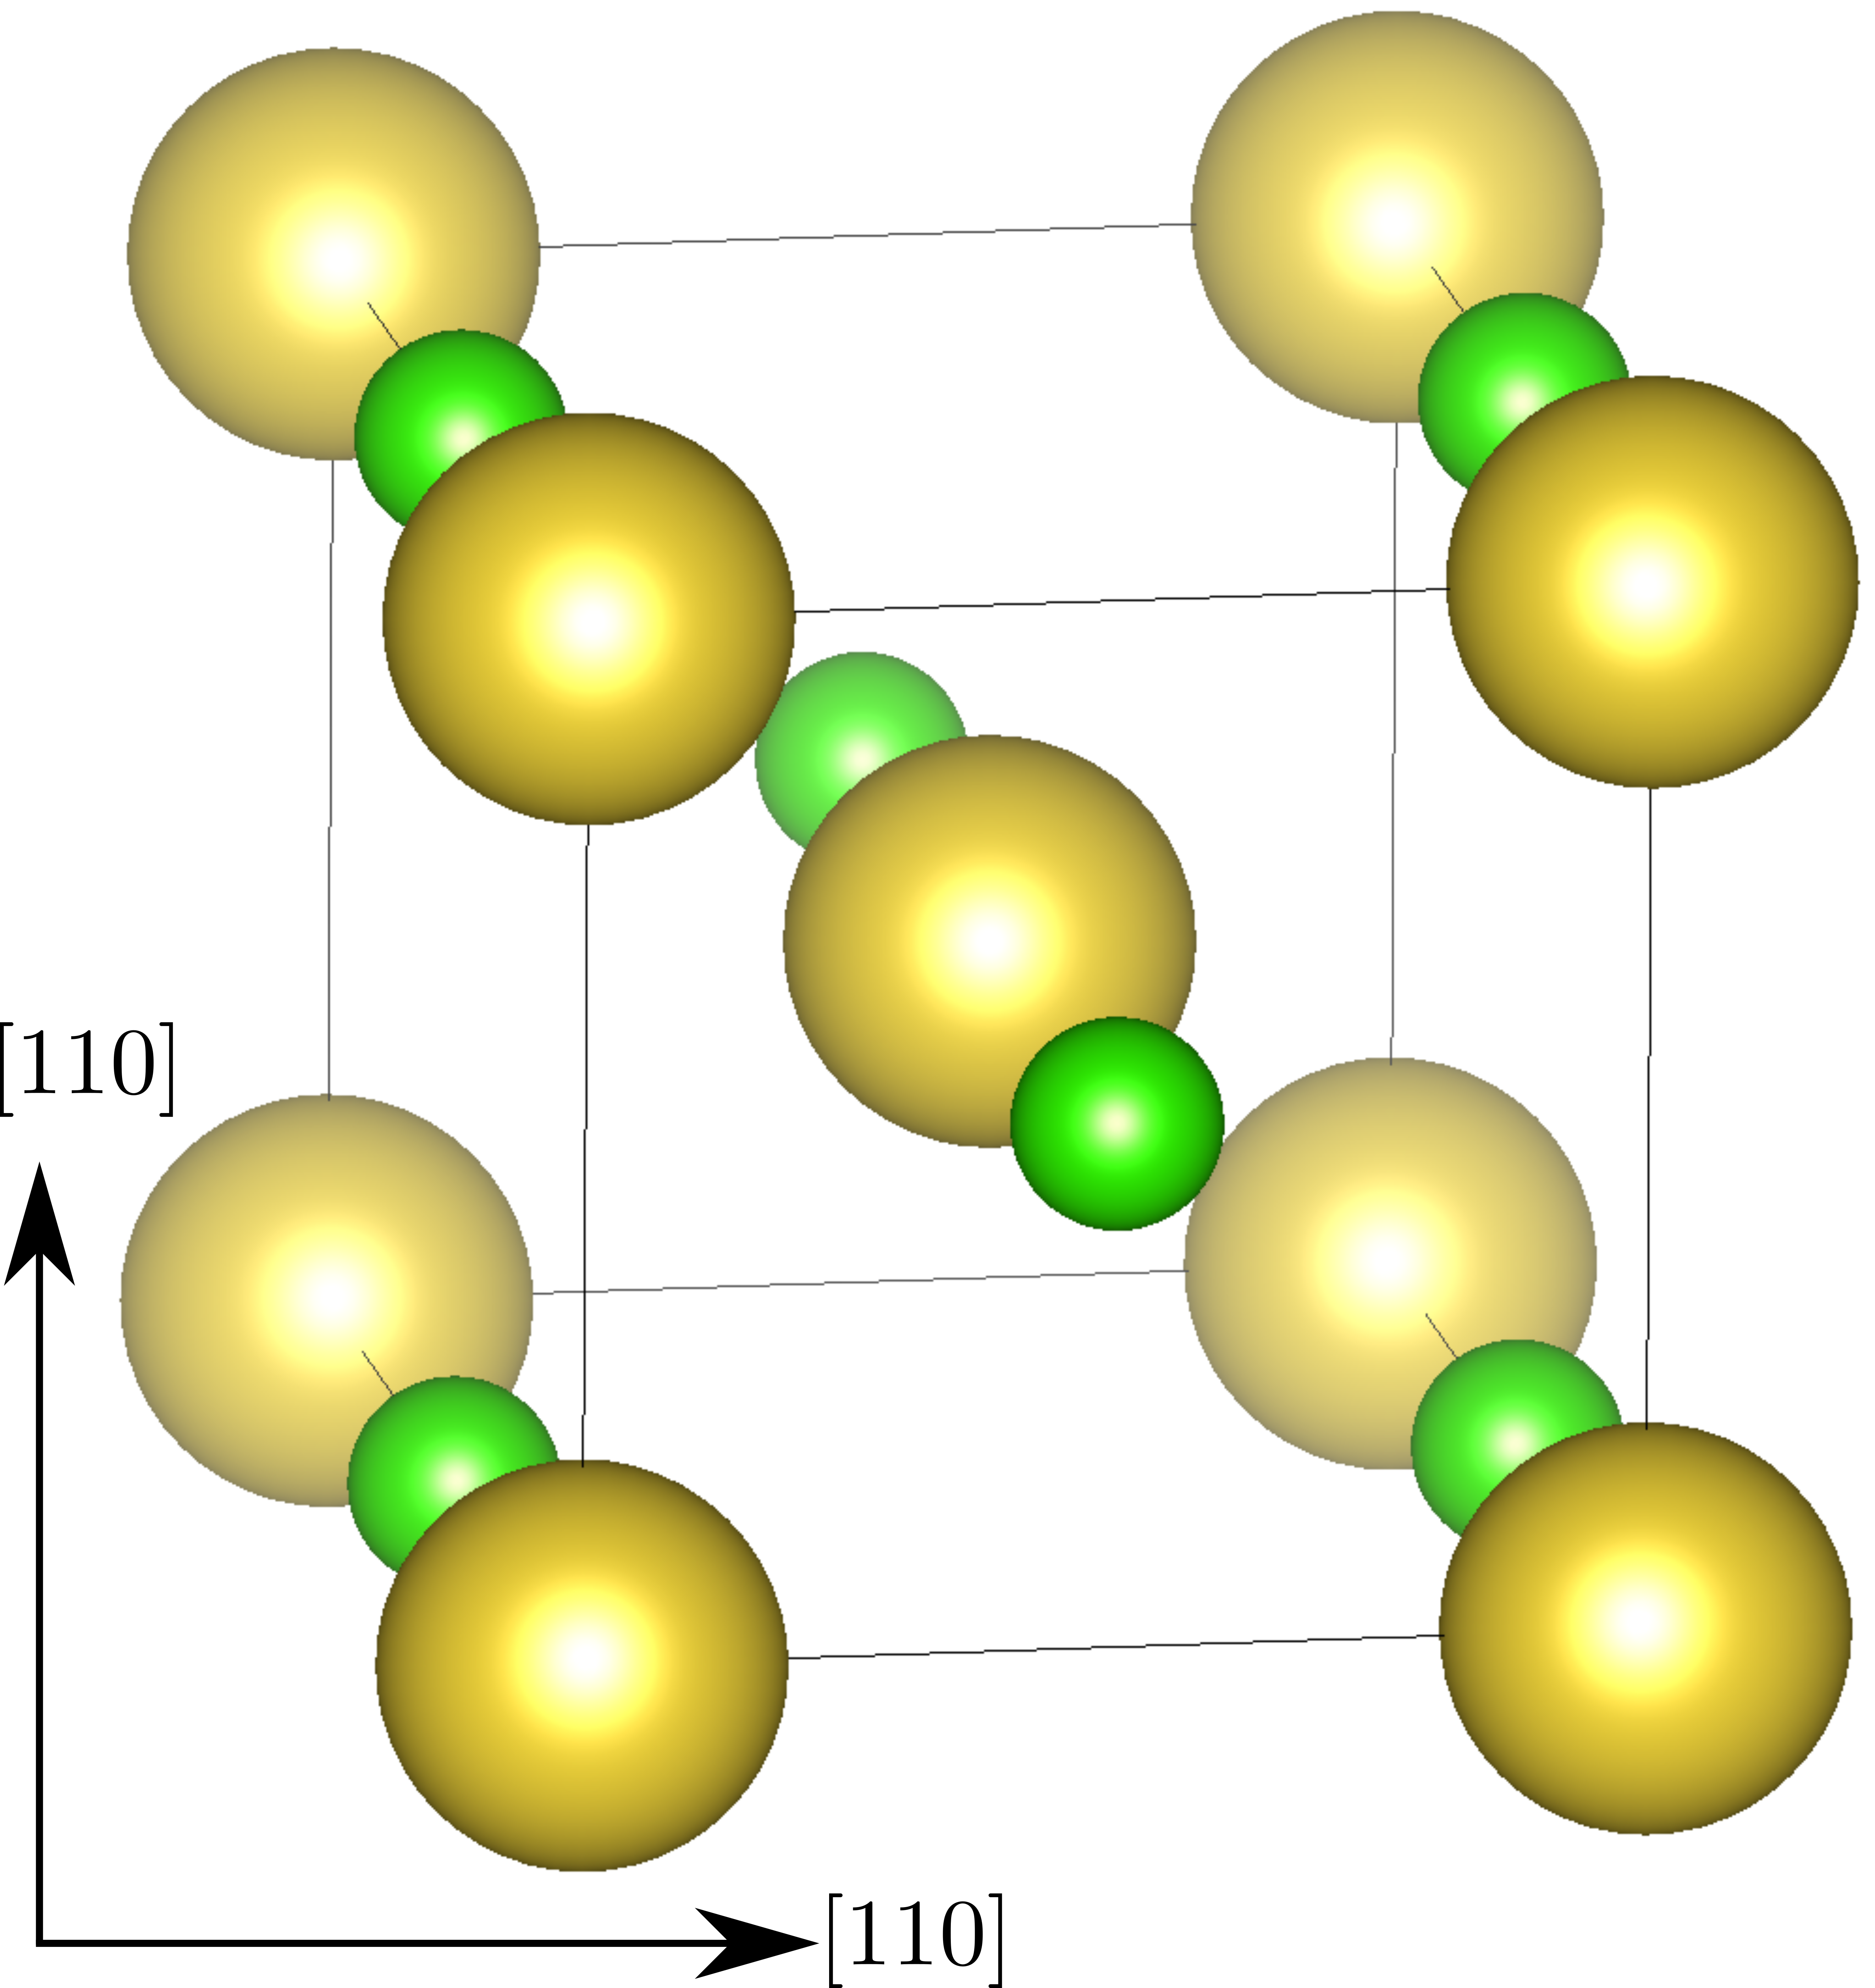
\includegraphics[height=2.0in]{NaCl_110_110_w_axes}
    \caption{The sodium chloride unit cell best aligned with the <110>\{1\={1}0\} slip system. \label{fig:NaCl_110_110_unit_cell}}
    \end{subfigure}
    ~
    \begin{subfigure}{0.4\textwidth}
    \centering
    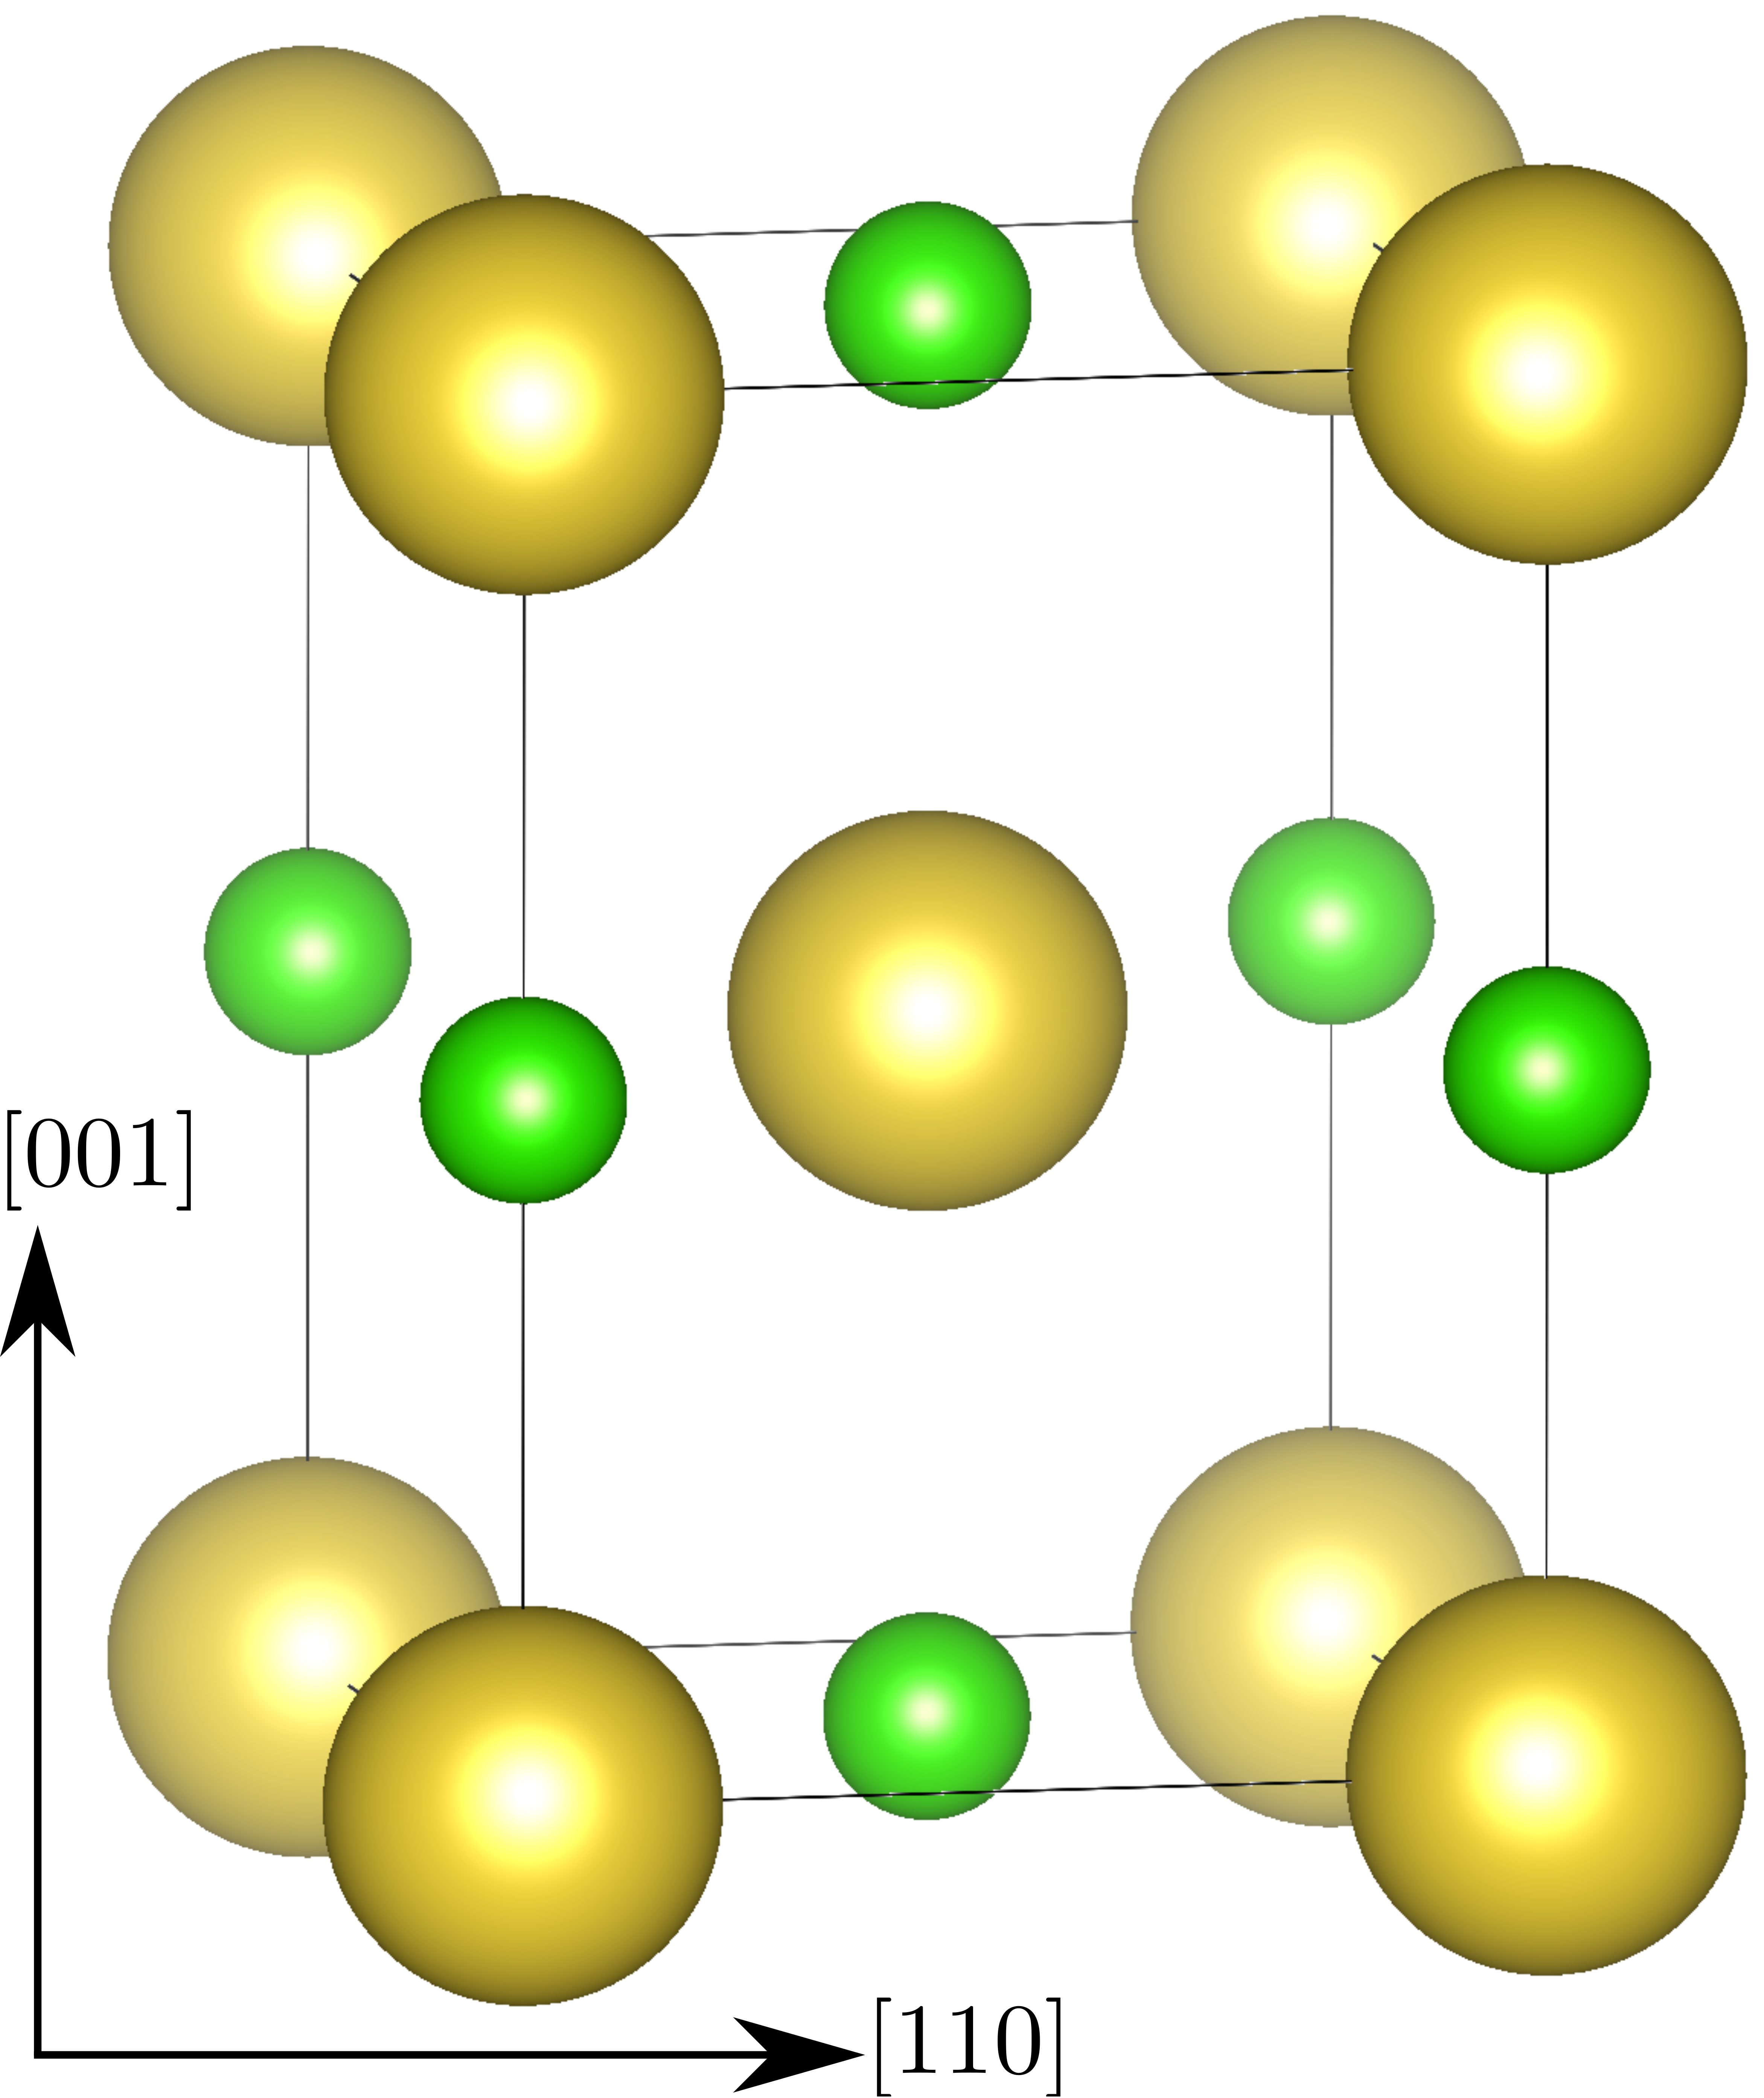
\includegraphics[height=2.5in]{NaCl_110_001_w_axes}
    \caption{The sodium chloride unit cell best aligned with the <110>\{001\} slip system. \label{fig:NaCl_110_001_unit_cell}}
    \end{subfigure}

\caption{Possible unit cells for sodium chloride showing the conventional unit cell and two unconventional unit cells with the new crystallographic axes aligned to slip system, i.e. the Burgers vector and slip plane normal.\label{fig:unconventional_NaCl_unit_cells}}
\end{figure}






Similarly the \ce{NaCl} <1\={1}0>\{001\} slip system is defined by the unit cell:

\begin{equation*}
\begin{aligned}[c]
 {[100]}' &=\, ^{1}\!/_{2} [110] \\
 {[010]}' &=\,  [001] \\
 {[001]}' &=\; ^{1}\!/_{2} [1\overline{1}0] \\
\end{aligned}
\qquad
\begin{aligned}[c]
&\parallel \mathbf{b} \\
&\parallel \mathbf{d} \\
&\parallel \mathbf{l}
\end{aligned}
\end{equation*}


and a possible new motif is 
$$
motif = \begin{pmatrix}
0 & 0 & 0 & +1 \\
^{1}\!/_{2} & ^{1}\!/_{2} & ^{1}\!/_{2} & +1 \\
^{1}\!/_{2} & 0 & ^{1}\!/_{2} & -1 \\
0 & ^{1}\!/_{2} & 0 & -1
\end{pmatrix}
$$


These unit cells are shown in relation to the conventional cell in \autoref{fig:unconventional_NaCl_unit_cells}. With these unit cells we can convolve the motif with a lattice to generate an initially perfect crystal defined with respect to Cartesian axes aligned with the slip system. Two offsets are then applied; firstly the half crystal below the slip plane, which is conveniently defined by $y < 0$, will be offset in the positive $x$ direction by $b/2$ and then the entire crystal is offset to put the dislocation core in the desired location. The latter will require an offset along the slip direction, $[001]'$ of $\alpha b$ and an additional offset in the $[010]'$. While the magnitude of this offset is not necessarily obvious in the case of \ce{NaCl} is fairly obviously that the core must be at a height of $d/4$ in order to be halfway between the two (020) layers.


Clearly in some crystals there will be multiple potential planes at different ``heights'' in the slip plane normal direction that the dislocation may glide along; some planes may be discarded as obviously energetically unfavourable or as being symmetrically equivalent but if the position the dislocation core will take is not obvious then a trial must be made of the all the plausible positions. Hence in addition to sampling a range of positions in the $[100]'$ direction, as characterised by $\alpha$, samples may be necessary in the $[010]'$ direction, characterised by a height $h$.

So the initial positions are related to those of an initially perfect crystal by
\begin{equation}
\bm{r_i^0} = \bm{r_i^{\text{perfect}}} +\begin{cases}
[-\alpha{}b, h, 0] & \quad \text{if } y_i^{\text{perfect}} > 0\\
[b(1/2 - \alpha{}), h, 0] & \quad \text{if } y_i^{\text{perfect}} < 0\\
\end{cases} 
\end{equation}

The offset to the atomic coordinates in $-\alpha{}b$ such that as $\alpha$ increases the dislocation motion is in the positive $x$ direction.





\FloatBarrier












%%%%%%%%%%%%%%%%%%%%%%%%%%%%%%%%%%%%%%%%%%%%%%%%%%%%%%%%%%%%%%%%%%%%%%%%%%%%%%%%%%%

                          % Displacement fields

\subsection{Displacement fields}

The choice of displacement field is obviously important but there is an obvious first guess: A Volterra dislocation in a continuous isotropic elastic medium has a displacement field \cite{hirth_lothe1982volterra_displacements}:
\begin{subequations}
\begin{align}
u^x &= \frac{b}{2\pi}\left[ \arctan\left(\frac{x}{y}\right) + \frac{xy}{2(1-\nu)(x^2 + y^2)} \right] \\[0.5ex]
v^y &= -\frac{b}{2\pi} \left[ \frac{1-2\nu}{4(1-\nu)} \ln(x^2 + y^2) + \frac{x^2 + y^2}{4(1-\nu)(x^2 + y^2)} \right]
\end{align}
\end{subequations}
Where $u^x$ and $v^y$ are the components of the displacement field parallel to $x$ and $y$ respectively, $x$ is the coordinate parallel to the Burgers vector and $y$ is the coordinate parallel to the slip plane normal, $b$ is the magnitude of the Burgers vector and $\nu$ is the Poisson ratio of the material. The terms all converge to fixed values at large $x$ or $y$ except the logarithmic dependence of $v^y$. This is physically reasonable and represents the bending of a single crystal that arises from the introduction of an extra half plane \cite{hirth_lothe1982volterra_displacements}.

This formulation of the stress field and subsequent solution for an isotropic elastic continuum is discontinuous, diverging at $r=0$, where $r=\sqrt[]{x^2+y^2}$. To remove the discontinuity \citet{Eshelby1949} proposed considering a single dislocation to instead be composed of a continuous distribution of dislocations with infinitesimal Burgers vectors, the integral of which yields the Burgers vector of the full dislocation. If $\bm{b}'(x')\mathrm{d}x'$ is the Burgers vector of an infinitesimal dislocation between $x'$ and $x'+\mathrm{d} x'$, and displacements in $y$ are assumed to be small, this can be related to the displacement, $u^x$, since the local displacement will be given by $-2(\mathrm{d} u^x/\mathrm{d} x)\mathrm{d} x'$ \cite{hirth_lothe1982peierls_displacements} we can write


\begin{equation}
b = \int_{-\infty}^{\infty} b'(x') \dd x' = -2\int^{\infty}_{-\infty} \left( \! \frac{\dd u^x}{\dd x} \right)_{x=x'} \dd x' 
\end{equation}

Using the result for a single volterra dislocation \cite{hirth_lothe_1982_volterra_stress_field}:

\begin{equation}
\sigma^{\text{volterra}}_{xy} = \frac{\mu b}{2\pi (1-\nu)} \frac{x(x^2 - y^2)}{(x^2+y^2)^2}
\end{equation}

and setting $y=0$

\begin{equation}
\sigma^{\text{volterra}}_{xy}(x,0) = -\frac{\mu}{2\pi(1-\nu)} \int^{\infty}_{-\infty} \frac{b'}{x-x'} \!\dd x' =  \frac{\mu}{\pi(1-\nu)} \int^{\infty}_{-\infty} \frac{1}{x-x'} \left(\!\frac{\dd u^x}{\dd x}\right)_{x=x'} \!\dd x'
\label{eqn:elastic_stress_at_slip_plane}
\end{equation}

At equilibrium the net stress at $(x,0)$ vanishes, so there must be a balancing stress arising from the misalignment of the material across the slip plane. By analogy with \citet{Frenkel1926}
\begin{equation}
\sigma_{xy}^{\text{misalignment}}(x,0) = C \sin \left( \frac{2\pi \phi^x}{b} \right)
\end{equation}
or in terms of the displacements either side of the slip plane:
\begin{equation}
\sigma_{xy}^{\text{misalignment}}(x,0) = -C \sin \left( \frac{4\pi u^x}{b} \right)
\end{equation}
By requiring Hooke's law to be satisfied at small strains we can write
\begin{equation}
\sigma_{xy}^{\text{misalignment}}(x,0) = 2 \mu \varepsilon_{xy} = \frac{\mu{}\phi^x}{d}
\label{eqn:misalign_stress_at_slip_plane}
\end{equation}
We can combine \autoref{eqn:elastic_stress_at_slip_plane} and \autoref{eqn:misalign_stress_at_slip_plane} to give a integral equation thus:
\begin{equation}
\int^{\infty}_{-\infty} \frac{1}{x-x'} \left(\!\frac{\dd u^x}{\dd x}\right)_{x=x'} \dd x' = \frac{b(1-\nu)}{2d} \sin\left(\frac{4\pi{}u^x}{b}\right)
\end{equation}
The solution is \cite{hirth_lothe1982peierls_displacements,Eshelby1949}
\begin{equation}
u^x(x) = -\frac{b}{2\pi} \arctan \left( \frac{x}{w} \right)
\label{eqn:one_dimensional_displacements}
\end{equation}
where $w$ is the half width of the dislocation and has the value
\begin{equation}
w = \frac{d}{2(1-\nu)}.\label{eqn:half_width}
\end{equation}
\autoref{eqn:one_dimensional_displacements} satisfies the boundary condition that $u^x(\infty) = - u^x(-\infty) = -b/4$. Also $x=w$ gives $u^x(w)=1/2\, u^x(\infty)$, i.e. in the region $-w < x < w$ the disregistry across the slip plane is greater than half the maximum that occurs at $x=0$.

A more generalised two dimensional case following a similar logic gives a full displacement field \cite{Eshelby1949,Leibfried1949,nabarro1987theory}
\begin{subequations}\label{eqn:displacements}
\begin{align}
u^x(x,y) &= \frac{b}{2\pi} \left( \arctan \left[ \frac{y +  w\frac{|y|}{y}}{x} \right] - \frac{\pi}{2} \frac{|y|}{y} \frac{|x|}{x} \right) + c_1 \frac{xy}{x^{2} + (y + w\frac{|y|}{y} )^2} \\
v^y(x,y) &= c_2 \frac{y(y +  w \frac{|y|}{y})}{x^2 + (y +  w \frac{|y|}{y})^2} + c_3 \ln \left| \frac{x^2 + (y +  w \frac{|y|}{y})^2}{b^2} \right|
\end{align}
\end{subequations}
So that the final atomic configuration is defined by 
\begin{equation}
\bm{r}_i = \bm{r}_i^0 + [u_i^x\,\bm{\mathrm{\hat{i}}},\; v_i^y\,\bm{\mathrm{\hat{j}}},\; 0\,\bm{\mathrm{\hat{k}}}]
\end{equation}



For an isotropic elastic medium the half-width, $w$, takes the same value as in \autoref{eqn:half_width} and the three other constants have defined values:
\begin{subequations}\label{eqn:disloc_params}
\begin{align}
c_1 &= \frac{b}{4\pi{}(1-\nu)} \\
c_2 &= \frac{b}{4\pi{}(1-\nu)} \\
c_3 &= - \frac{b(1-2\nu)}{8\pi(1-\nu)}.
\end{align}
\end{subequations}
The terms of the form $|x|/x$ and $|y|/y$ are simply to give all the terms the right sense in the right regions of space, i.e. above and below the slip plane in $y$ and either side of the dislocation in $x$. This reduces to the simpler solution in \autoref{eqn:one_dimensional_displacements} if only the atoms adjacent to the slip plane are considered. This form is useful because it is continuous and finite for all values of $x$ and $y$. 



\begin{figure}
\centering

    \begin{subfigure}{0.4\textwidth}
    \centering
    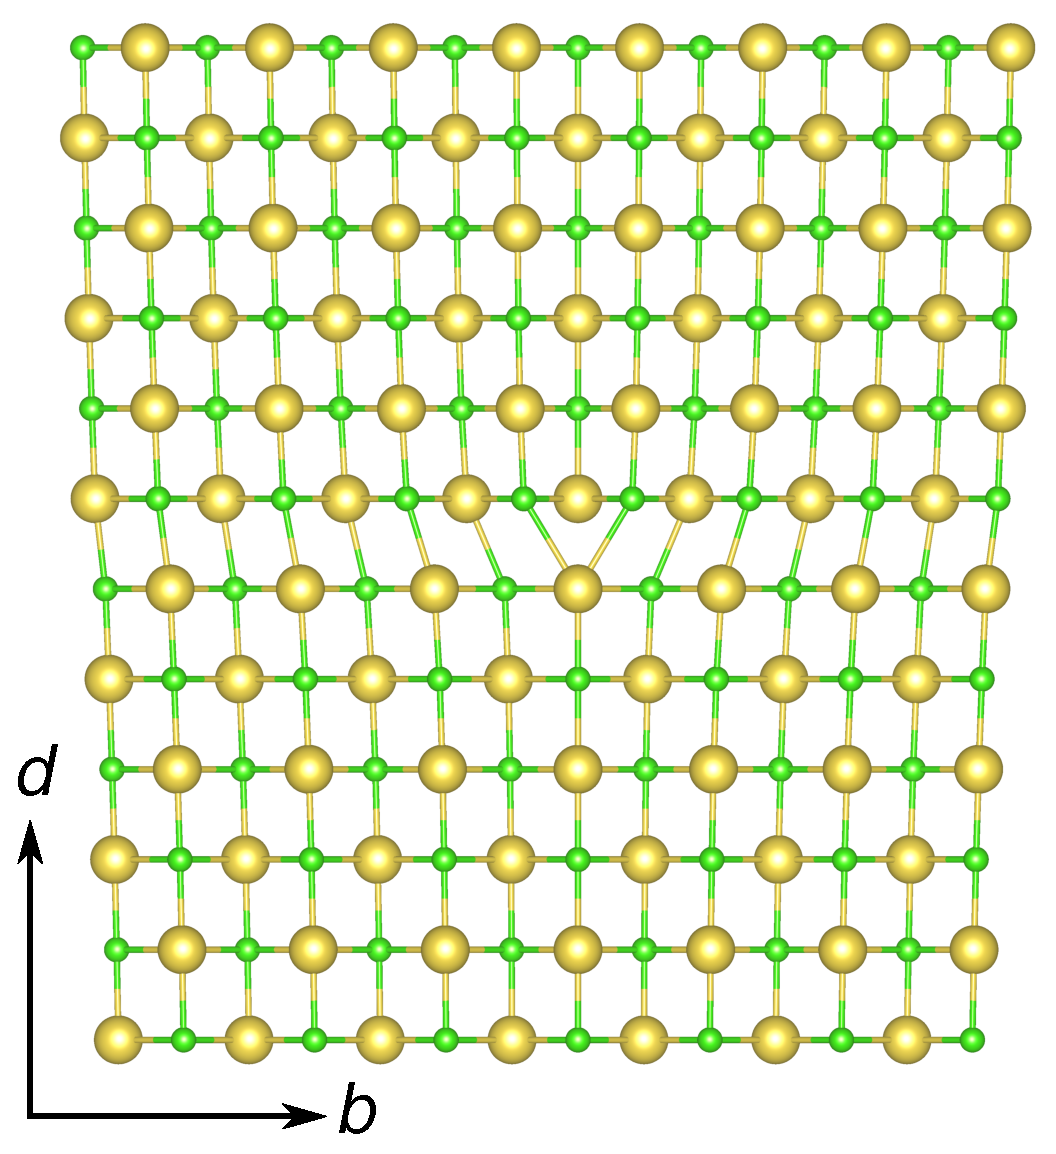
\includegraphics[width=0.6\textwidth]{wide_NaCl}
    \caption{A dislocation with a large width.}
    \end{subfigure}
    ~
    \begin{subfigure}{0.4\textwidth}
    \centering
    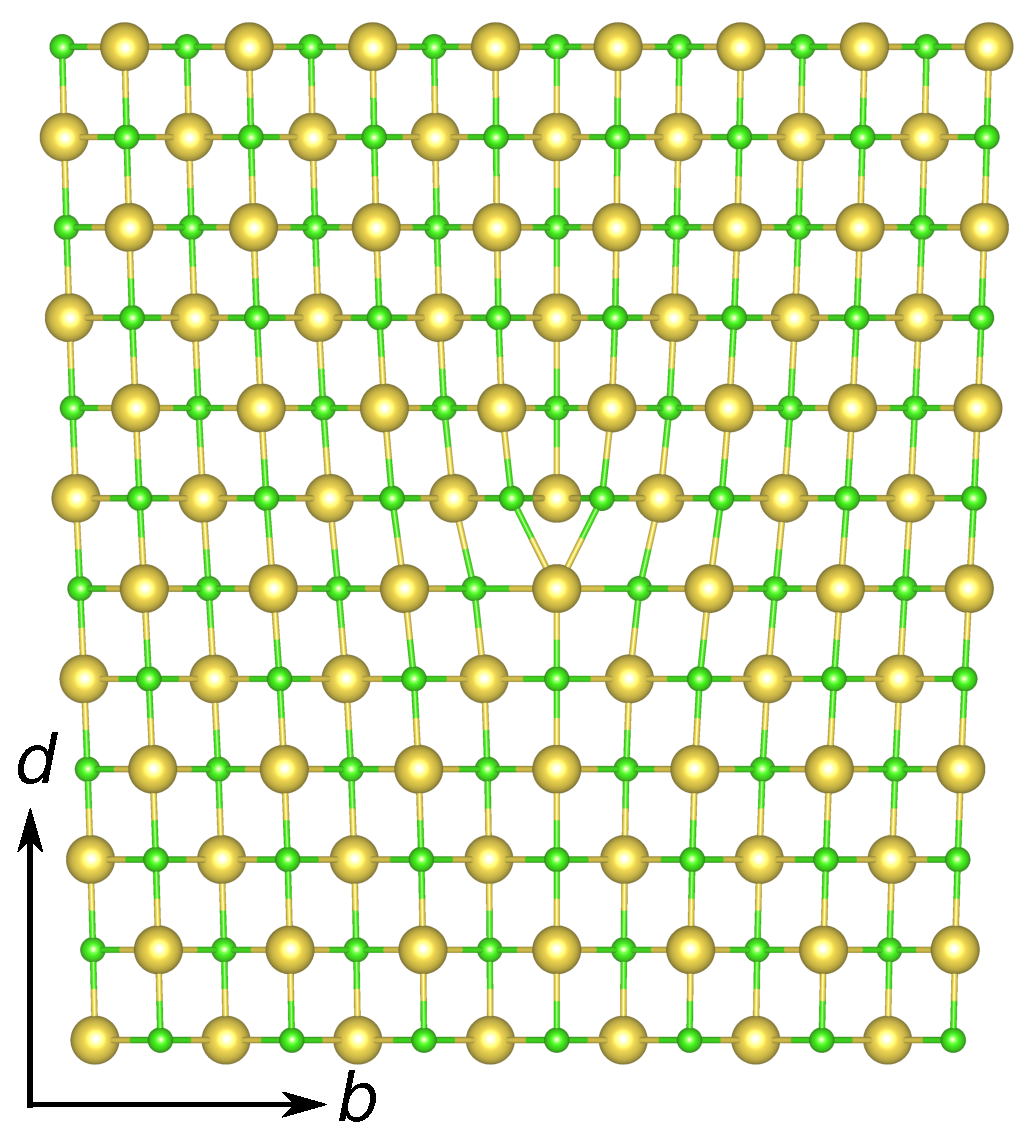
\includegraphics[width=0.6\textwidth]{narrow_NaCl}
    \caption{A dislocation with a small width.}
    \end{subfigure}

	\begin{subfigure}{0.4\textwidth}
	\centering
    \includegraphics[width=0.6\textwidth]{large_c1_NaCl}
    \caption{Large values of $c_1$ and $c_2$.}
	\end{subfigure}
    ~
	\begin{subfigure}{0.4\textwidth}
	\centering
    \includegraphics[width=0.6\textwidth]{large_c3_NaCl}
    \caption{A large value of $c_3$.}
	\end{subfigure}

    \begin{subfigure}{0.8\textwidth}
    \centering
    \includegraphics[width=0.5\textwidth]{typical_NaCl}
    \caption{A ``typical'' configuration.}
    \end{subfigure}

\caption{Various configurations of sodium chloride <110>\{001\} dislocations demonstrating the effects of the parameters of the displacement field defined in \autoref{eqn:displacements}, $w$, $c_1$, $c_2$ and $c_3$. Typical parameters are taken to be those predicted for an isotropic elastic material as given in  Equations~\ref{eqn:half_width} and \ref{eqn:disloc_params}. To illustrate $c_1$, $c_2$ and $c_3$ a ``typical'' value of $w=$~\SI{1.03}{\angstrom} was used, assuming $\nu =$~\num{0.207} \cite{Theocaris1994}.\label{fig:parameters_of_the_disloc_configuration}}
\end{figure}


This provides a parametrised displacement field for a general material in which the width, $w$, and the constants, $c_1$, $c_2$ and $c_3$ are allowed to vary. The width of the dislocation still defines the region with large disregistries (or equivalently small displacements), while $c_1$ and $c_2$ define the magnitude of displacements associated with shear strains around the dislocation core and $c_3$ defines the bending of a crystal that must arise from the introduction of an extra half plane.
To illustrate the displacements produced by these different terms some exaggerated dislocation configurations are shown in \autoref{fig:parameters_of_the_disloc_configuration}.





A final note on the parametrisation of the dislocation structure is that the values $c_1$, $c_2$ and $c_3$ are not constrained, while they have expected signs and magnitudes based on the purely isotropic elastic results described above there is no physical reason they cannot be negative however a negative value of the width reintroduces the discontinuity at which displacements would diverge (in fact it would introduce two, one in each half crystal) which cannot be the case. Hence the constraint that $w>0$ is applied, but $c_1$, $c_2$ and $c_3$ are allowed to vary freely.


\section{Evaluating the dislocation energy}




Since there are insufficient boundary conditions to completely define a dislocation configuration with even four parameters the energy of the dislocation is the only way to identify a``correct'' or true configuration. Hence we must characterise the energy of arbitrary configurations. One obvious method to calculate the energy is to try and replicate the model based on elastic energy in the two half crystals and misalignment energy across the slip plane, there is the opportunity to calculate the full strain tensor and along with single crystal elastic constants the effects of elastic anisotropy can be taken into account. Another would be to use empirical potentials similar to those used in molecular dynamics; this would allow the exploration of dislocation properties in materials that are not well modelled by elasticity, ionic solids or compound semiconductors are examples of materials where elasticity is probably less appropriate. Both of these approaches are explored.

\subsection{Strain energy and misalignment energy}

This is building on the original approach of \citet{Peierls1940} and then \citet{Nabarro1947} and explains how the dislocation is stable due to a balancing of two forces, there is a force that attempts to spread teh dislocation out into a planar defect, this arises due to the elastic stored energy in the bonds either side of the slip plane which would be zero in the case of a planar defect, which can be described by an infinitely wide dislocation. The other force tends to narrow the dislocation, this arises due to the misfit or misalignment across the slip plane. This would be a maximum for the planar defect where the entire slip plane is misaligned and would decrease monotonically as the width decreases.

Using this approach to the energy has a number of advantages. A two dimensional model is sufficient since for a long dislocation the condition of plane strain can be applied. If elastic theory can be applied at the scale of the unit cell then displacements need only be considered between unit cells rather than within them, which simplifies the model considerably.

\subsubsection{Strain energy}

Firstly the elastic energy can be easily calculated for a small volume if the strain and the elastic tensor is known. A good discussion of tensors and elasticity is given by \citet{kelly_knowles2012chapter5_tensors,kelly_knowles2012chapter6_stress_strain} and a discussion of elasticity in the context of dislocation theory is given by \citet{hirth_lothe1982elasticity}. The salient results are drawn together here.

Hookes law can be written as a tensor relationship using the einstein summation convention:
\begin{equation}
\sigma_{ij} = c_{ijkl} \epsilon_{kl}
\end{equation}
where $\sigma_{ij}$ is the stress tensor, $c_{ijkl}$ is the elastic tensor defining the properties of the material and $\epsilon_{kl}$ is the strain tensor. Strain is defined, for $i=j$, by
\begin{equation}
\epsilon_{ii} = \frac{\partial u_i}{\partial x_i}
\end{equation}
and for $i\neq j$ by
\begin{equation}
\epsilon_{ij} = \frac{1}{2} \left( \frac{\partial u_i}{\partial x_j} + \frac{\partial u_j}{\partial x_i} \right)
\end{equation}

%In Voigt notation the equation can be written
%\begin{equation}
%\sigma_i = c_{ij} \epsilon_{j}
%\end{equation}
%where 
%\begin{equation}
%\sigma_i = \begin{bmatrix}
%\sigma_{11} \\
%\sigma_{22} \\
%\sigma_{33} \\
%\sigma_{23} \\
%\sigma_{31} \\
%\sigma_{12} 
%\end{bmatrix}
%\qquad\qquad
%\epsilon_i = \begin{bmatrix}
%\epsilon_{11} \\
%\epsilon_{22} \\
%\epsilon_{33} \\
%\gamma_{23} \\
%\gamma_{31} \\
%\gamma_{12} 
%\end{bmatrix}
%\end{equation}
%This allows the reduction of the $3\times3\times3\times3$ tensor $c_{ijkl}$ to a $6\times6$ matrix $c_{ij}$. Note that to preserve the symmetry across the leading diagonal in $c_{ij}$ the strain components for $i\neq j$ are defined by $\gamma_{ij} = 2 \epsilon_{ij}$.


If Hooke's law holds then the stored elastic energy per unit volume is
\begin{equation}
u_{\text{elastic}} =\, ^{1}\!/_{2}\, \sigma_{ij} \epsilon_{ij} =\, ^{1}\!/_{2}\, c_{ijkl} \epsilon_{ij} \epsilon_{kl}.
\end{equation}
Hence to find the elastic energy we must evaluate \({\partial u_i}/{\partial x_j}\) for $i, j = 1, 2, 3$.
Assuming that we consider displacements between unit cells, and not within them, and assuming an orthogonal lattice estimating the components of strain is not difficult. The  condition of plane strain constrains $\epsilon_{ij} = 0$ for $i\, \text{or}\, j=3$. In the $1$--$2$ (or $x$--$y$) plane the strains can be identified from the vectors between neighbouring unit cells. For simplicity a primitive lattice is assumed and these vectors can be conceived of as bonds.

For this simple case for each atom two bonds are identified, one to the nearest neighbour in the $x$~direction and one to the nearest neighbour in the $y$~direction as shown in \autoref{fig:bonds}. The simplest estimate of the  stress components is

\begin{figure}
\centering
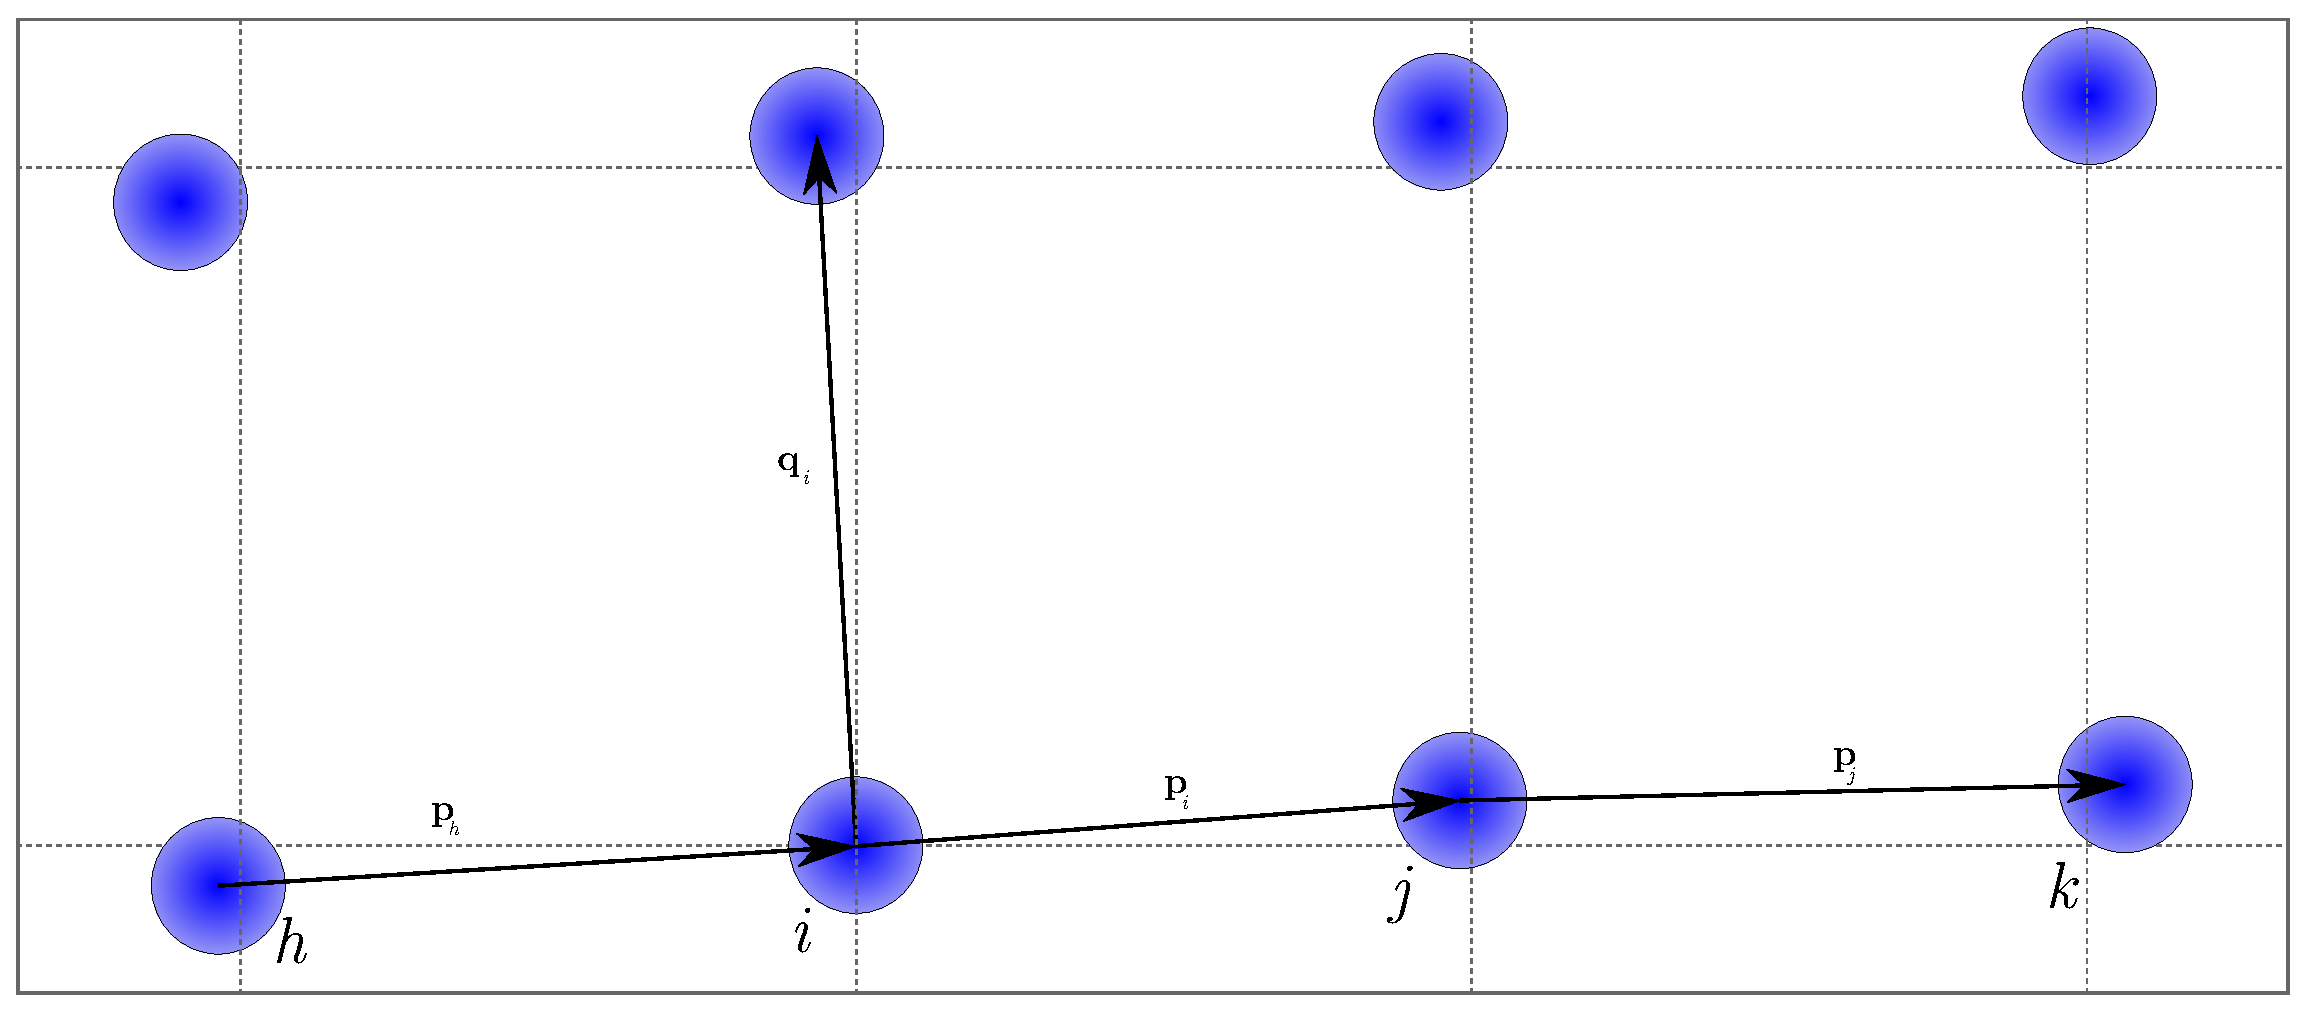
\includegraphics[width=\textwidth]{bonds}
\caption{The bonds that are considered for the $i$th atom, one to the nearest neighbour in the positive $x$~direction, $\mathbf{p}_i$, and one to the nearest neighbour in the positive $y$~direction, $\mathbf{q}_i$.\label{fig:bonds} }
\end{figure}




\begin{alignat}{2}\label{eqn:estimate_strains}
\left. \frac{\partial u_x}{\partial x}\right|_i &= \frac{\mathbf{p}_i \cdot \mathbf{\hat{i}}}{b} &\qquad\qquad
\left. \frac{\partial u_x}{\partial y}\right|_i &= \frac{\mathbf{q}_i \cdot \mathbf{\hat{i}}}{d} \nonumber\\
\left. \frac{\partial u_y}{\partial y}\right|_i &= \frac{\mathbf{q}_i \cdot \mathbf{\hat{j}}}{d} &
\left. \frac{\partial u_y}{\partial x}\right|_i &= \frac{\mathbf{p}_i \cdot \mathbf{\hat{j}}}{b}
\end{alignat}


However there is a problem with this formulation. This assumes that every bond would, in equilibrium, be parallel to either the $x$ or the $y$ axis. This assumption is valid for the original Peierls model in which only displacements parallel to the $x$ direction were considered but the logarithmic term here represents a change in lattice orientation with position. A more nuanced approach requires some estimate of the local lattice orientation, if this is not done then the logarithmic term in \autoref{eqn:displacements} will mean that the strain in each bond will diverge, increasing with increasing distance from the dislocation core, whereas in reality the strains must be largest at the core.

There are clearly many possible ways of estimating the local lattice resistance, one possible method is to take the ideal orientation of the bond parallel to the slip plane for a particular bond to be paralell to the bonds on either side, i.e. as shown in \autoref{fig:bonds} the ideal orientation of $\mathbf{p}_i$ would be  parallel to $(\mathbf{p}_h + \mathbf{p}_j)$. The ideal orientation for $\mathbf{q}_i$ can be taken to be at \SI{90}{\degree} to this. So $\mathbf{\hat{i}}$ and $\mathbf{\hat{j}}$ in \autoref{eqn:estimate_strains} can be replaced with 
\begin{align}
\mathbf{\hat{i}}' &= \frac{(\mathbf{p}_h + \mathbf{p}_j)}{|\mathbf{p}_h + \mathbf{p}_j|} \nonumber \\
\mathbf{\hat{j}}' &= {\mathbf{\hat{i}}' \times \mathbf{\hat{k}}}
\end{align}
and the strain tensor can be calculated for each atom/unit cell, and hence the strain energy for each unit cell.



\FloatBarrier
\subsubsection{Misalignment energy}
\FloatBarrier
At the slip plane there is clearly going to be a break down of method highlighted above. For an atom immediately below the slip plane the identification of the nearest neighbour above the slip plane is perhaps not obvious. If the bond is taken to be simply  to the nearest atom above the slip plane ambiguities can arise 
It is possible that there will be two atoms equally close above the slip plane and such a simple criterion can lead to some atoms being bonded more than once and some atoms not being bonded. 

Instead a less arbitrary and more predictable method is to use the initial positions and assume that the $i$th atom can be bonded to two atoms in the layer above the slip plane. Since initially the horizontal spacing between atoms is $b$ for all atoms the two atoms must be within an interval $x_i^0 - b < x \leq x_i^0 + b$, as shown in \autoref{fig:slip_plane}. The energy for atom $i$ can be estimated from the average of the two bonds $\mathbf{q}_{i,\text{b}}$ and $\mathbf{q}_{i,\text{f}}$

\begin{figure}
\centering
\begin{subfigure}{\textwidth}
\centering
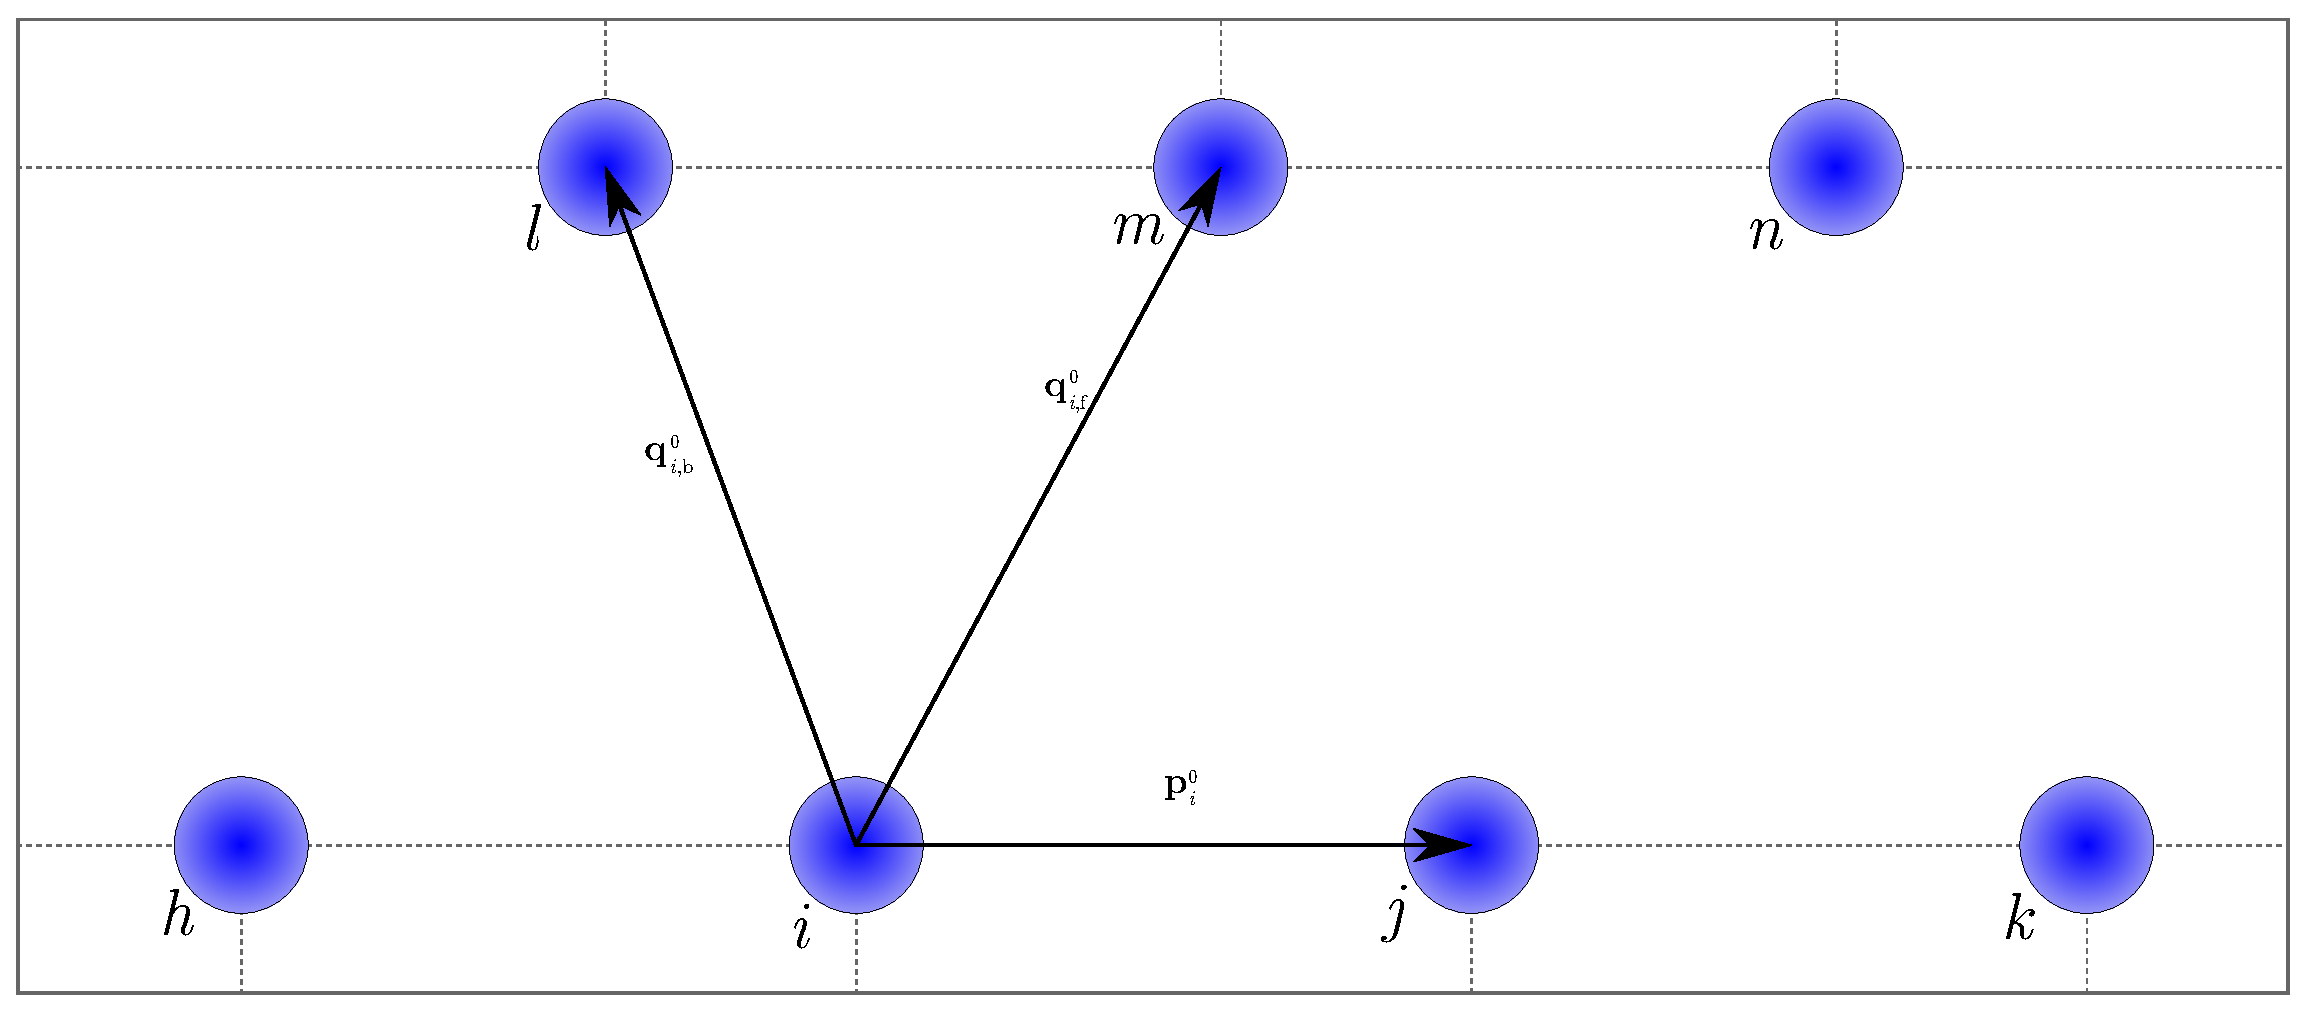
\includegraphics[width=\textwidth]{initial_slip_plane_bonds}
\caption{The initial positions of atoms either side of the slip plane.\label{fig:slip_plane_initial_positions}.}
\end{subfigure}
\par\medskip
\begin{subfigure}{\textwidth}
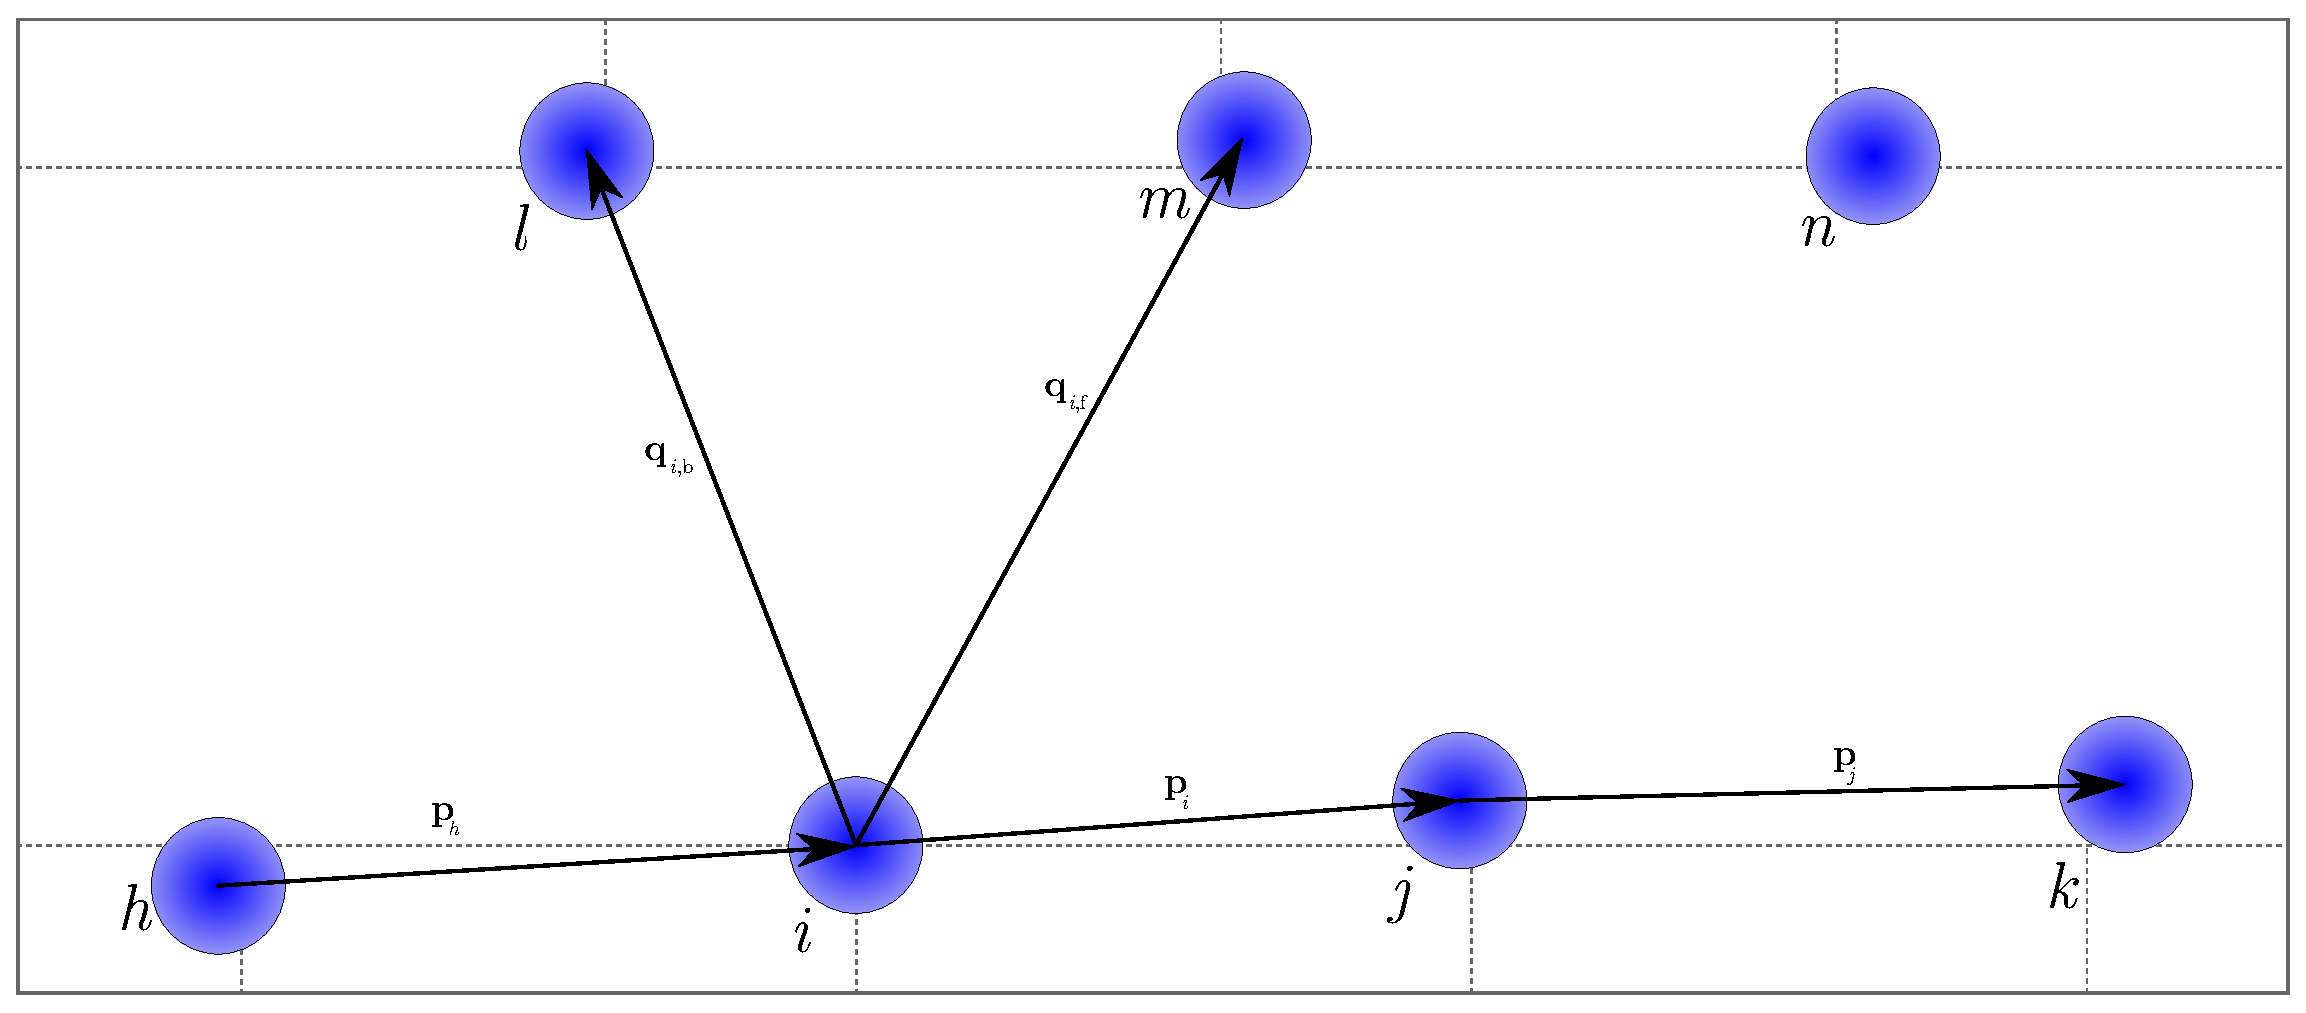
\includegraphics[width=\textwidth]{slip_plane_bonds}
\caption{The final positions of the atoms either side of the slip plane.\label{fig:slip_plane_final_positions}}
\end{subfigure}
\caption{The slip plane before and after the application of the displacement field. The two atoms, $l$ and $m$, that can be considered bonded to the atom $i$ are shown along with the initial and final bonds, $\mathbf{q}_{i,\text{b}}$ and $\mathbf{q}_{i,\text{f}}$ which are backwards and forwards in the $x$ direction respectively. Also shown are the bonds $\mathbf{p}_h$ and $\mathbf{p}_j$ which are required to estimate the local orientation of the slip plane. \label{fig:slip_plane}}
\end{figure}


There are several methods to calculate the misaligned bonds. The simplest is to use the Frenkel approximation which, for an isotropic elastic material is 
\begin{equation}
U_i^\text{mis} = \frac{Gb^2}{4\pi^2} \left[\frac{d}{b}\right] \left[ 1 - \cos \left( \frac{2 \pi \phi}{d} \right) \right]
\end{equation}

which in terms of single crystal elastic constants takes $G=C_{66}$ (in Voigt notation see \cite{kelly_knowles2012chapter6_stress_strain}).

A more complete method for the calculation of the energy is to use the generalised stacking fault energy.































%\chapter{Heterogeneity in the MAX phases}

\graphicspath{{Chapter3/Figs/}}


As  discussed in \autoref{sec:ductility_criteria} the MAX phases are predicted to be brittle by a wide range of ductility criteria but they are in fact observed to be damage tolerant and to flow easily in the basal plane \cite{Barsoum1999}.
Predictions of the Peierls stress made using the methods described in \autoref{sec:dislocations} have been made previously \cite{Music2007ductility,Gouriet2015}, however these have had limited success, producing over estimates, for example \citet{Gouriet2015} reported the Peierls stress to be at least \SI{611}{\mega\pascal} which is in fact slightly higher than that estimated for titanium carbide and other very hard brittle materials in which slip is limited at room temperature by the Peierls mechanism \cite{Chang1966,Clegg2006,Kamimura2011,Yadav2014}. Given that flow stresses in the region of a few tens of \si{\mega\pascal} have been observed at room temperature \cite{Humphrey2012,Barsoum1999}, which is more comparable with FCC metals than FCC carbides, it is reasonable to expect the Peierls stress to be lower than this.

The poor performance of Peierls models for MAX phases, and potentially for other complex phases, is possibly due to the treatment of the MAX phase unit cell as homogeneous elastically. This is surprising because many studies have discussed the heterogeneity of the bonding and electron structure, a recent review was written by \citet{Magnuson2017}, and discusses the complex and mixed nature of the bonding varying across the different atomic sites, more metallic in the MA layers, more covalent in the MX layers, and charge transfer contributing an ionic component to the bonding. Clearly this bonding is necessary for many of the MAX phases intriguing properties, e.g. high melting point, high specific stiffness, electrical and thermal conductivity, and a near zero Seebeck coefficient to name a few \cite{Yoo2000,Sun2011,Magnuson2017} but the clear and strong heterogeneity of the unit cell has largely been neglected when considering the dislocation properties of the MAX phases, the only account made for it being the choice of plane at which the generalised stacking fault energy was calculated.

If the MAX phases are elastically heterogeneous there is the uestion of what might be the expected properties and where within the MAX phase unit cell. A simple metric to characterise the chemical heterogeneity is the electronegativity, $\chi$, of regions within the unit cell. For both the M--X and M--A regions, an average electronegativity is easily calculated as once sharing of atoms between the regions is accounted for there are equal numbers of M and A atoms in the M--A region and similarly equal numbers of M and X atoms in the M--X region. The difference in electronegativity between the two regions is therefore defined by
\begin{equation}
\Delta \chi = \frac{\chi_{\text{X}} - \chi_{\text{A}}}{2}
\end{equation}
since the M atoms contribute to both regions. There are a variety of measures of electronegativity, but perhaps the most fundamental is the Mulliken scale \cite{Mulliken1934}, which takes the electronegativity of a species to be the average of the ionization energy, the energy change on removing an electron, and the electron affinity, the energy change on adding an electron. This scale is more fundamental than others because it is calculated from the fundamental properties of atoms, as opposed to more ``relative'' scales that are calculated from enthalpies of formation and covalent radii and so on \cite{huheey1983ch3_electronegativity}.

Since the elements that take the X site, carbon and nitrogen, are generally more electronegative than those that take the A site, elements like aluminium and silicon, it is expected that electron transfer into the M--X region from the M--A. Such a transfer would be expected to increase the strength of the bonding in the M--X layer and reduce it in the M--A, with a corresponding change in the modulus.

\section{Calculating the local stiffness}

Measuring single crystal elastic constants for the MAX phases is extremely difficult due to the difficulty of growing single crystals and experimentally determining the stiffness of sub-unit cell regions of the crystal presents an even greater challenge. Instead density functional theory can be employed. DFT has been widely used to calculate single crystal elastic constants of a large variety of materials and is considered reliable and reproducible \cite{Lejaeghere2016}. One commonly used method for calculating the elastic constants via DFT is simply to simulate the unit cell with periodic boundary conditions and apply a stress/strain state and fit either the equation
\begin{equation}
\sigma_{ij} = C_{ijkl} \epsilon_{kl}
\end{equation}
or 
\begin{equation}
u = \frac{1}{2} C_{ijkl} \epsilon_{ij} \epsilon_{kl}
\end{equation}
where $\sigma_{ij}$ is the stress tensor, $\epsilon_{ij}$ is the strain tensor, $u$ is the strain energy per unit volume and $C_{ijkl}$ is the stiffness tensor. This was applied by \citet{Aryal2014} to a very wide range of MAX phases. Care must be taken to reproduce the physically realistic situation where the stress is equal throughout the unit cell but the strain can vary, that is the strain must be applied macroscopically (i.e. to the simulation cell) but the atomic positions must be allowed to vary to find the lowest energy configuration.

The latter equation was used to find the local stiffness within a region of the unit cell. The single crystal elastic constants must be dropped since a tensor formulation of heterogeneous elasticity is not the aim, instead local shear moduli are calculated. The unit cell is divided naturally into two distinct regions that are obvious from the geometry of the crystal structure, the local chemistry and nature of bonding, there is a more metallic layer, the M--A layer, and a more covalent layer, the M--X layer, see \label{fig:fig:MAX_unit_cells}. The layer of M-atoms that are bonded to both A-atoms and X-atoms is the natural boundary.

To localise the strain in, say, the M--A layer all the bonding, that is the relative atomic positions, in the M--X layer are held rigid and are displaced as a whole such that in each M--A layer the appropriate strain is applied. The relative positions of the atoms within the M--A layer are then allowed to relax to achieve the minimum energy. The equation that must then be fitted is
\begin{equation}
u = \frac{1}{2} G_{i} \gamma^2
\end{equation}
where $\gamma$ is the applied strain and $G_i$ is the local shear modulus, namely either $G_{M\text{--}A}$ or $G_{M\text{--}X}$. The procedure is applied vice versa to calculate the M--X properties.




\begin{figure}
\centering
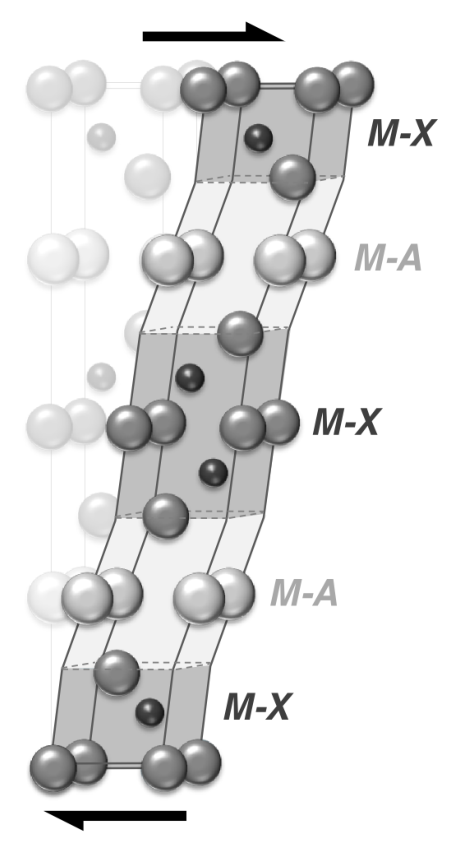
\includegraphics[height=0.3\textheight]{slab_model}
\caption{Schematic of non-uniform elastic deformation in a ``211'' MAX phase showing the regions that might be considered distinct, the M--A and M--X layers.}
\end{figure}



The overall shear modulus for the whole crystal structure is calculated in the same manner with no restrictions on the atomic positions, all the atoms are allowed to relax fully. Since this relaxed shear is equivalent to a uniform applied stress an analogy is possible with the assumptions made to calculate the transverse stiffness of long fibre composite materials, the so called slab model \cite{Hull1996ch4}. The slab model is illustrated in . The results of the local calculations can be compared with the overall case using the equation:

\begin{equation}
G_{\text{slab}} = \left[ \frac{f_{M\text{--}X}}{G_{M\text{--}X}} + \frac{f_{M\text{--}A}}{G_{M\text{--}A}} \right]^{-1}
\end{equation}
where $G_{\text{slab}}$ is the estimate for the overall shear modulus, $f_i$ is the volume fraction of the region $i$ and $G_i$ is the shear modulus of region $i$. The volume fractions are estimated from the crystal structures of the MAX phases. In particular the fractional coordinate in the $c$ direction of the M1 site in the ``211'' phases, $z_1$, and the position of the M2 site in the ``312'' and ``413'' phases, $z_2$, as shown in \autoref{fig:MAX_unit_cells}, determines the volume fraction of the regions of the unit cell.













%\include{Chapter4/chapter4}
%\include{Chapter5/chapter5}
%\include{Chapter6/chapter6}
%\include{Chapter7/chapter7}




% ********************************** Back Matter *******************************
% Backmatter should be commented out, if you are using appendices after References
%\backmatter

% ********************************** Bibliography ******************************
\begin{spacing}{0.9}

% To use the conventional natbib style referencing
% Bibliography style previews: http://nodonn.tipido.net/bibstyle.php
% Reference styles: http://sites.stat.psu.edu/~surajit/present/bib.htm

\bibliographystyle{my_bib_style}
%\bibliographystyle{plainnat} % use this to have URLs listed in References
\cleardoublepage
\bibliography{references} % Path to your References.bib file


% If you would like to use BibLaTeX for your references, pass `custombib' as
% an option in the document class. The location of 'reference.bib' should be
% specified in the preamble.tex file in the custombib section.
% Comment out the lines related to natbib above and uncomment the following line.

%\printbibliography[heading=bibintoc, title={References}]


\end{spacing}

% ********************************** Appendices ********************************

\begin{appendices} % Using appendices environment for more functionality

%% ******************************* Thesis Appendix A ****************************

%% ******************************* Thesis Appendix B ********************************

\chapter{Installing the CUED class file}


\end{appendices}

% *************************************** Index ********************************
\printthesisindex % If index is present

\end{document}
